\documentclass[aspectratio=169,11pt]{beamer}

% Shared style (ib-tutorials.sty at the repo root).
\makeatletter\def\input@path{{./}{../}}\makeatother
\usepackage{ib-tutorials}

\usepackage[utf8]{inputenc}
\usepackage{amsmath,amssymb}
\usepackage{booktabs}
\usepackage{array}
\newcolumntype{L}[1]{>{\raggedright\arraybackslash}p{#1}}
\usepackage{graphicx}
\graphicspath{{../pictures/appendices/}{pictures/appendices/}}
\usepackage{xcolor}
\usepackage{listings}
\usepackage{tikz}
\usetikzlibrary{arrows.meta,positioning,shapes.geometric,fit,calc}
\usepackage{hyperref}

\newcommand{\sourcecredit}[1]{\vfill\begin{flushright}\tiny\textcolor{DarkGray}{#1}\end{flushright}}
\setbeamertemplate{itemize/enumerate body begin}{}
\setbeamersize{description width=3em}

\lstset{
  basicstyle=\ttfamily\scriptsize\color{BlackGray},
  keywordstyle=\color{NavyBlue}\bfseries,
  commentstyle=\color{DarkGray}\itshape,
  stringstyle=\color{OliveGreen},
  showstringspaces=false,
  columns=fullflexible,
  keepspaces=true,
  breaklines=true,
  breakindent=1em,
  frame=single,
  framerule=0.4pt,
  rulecolor=\color{LightGray},
  backgroundcolor=\color{LightGray!30},
  xleftmargin=0.25em,
  xrightmargin=0.25em
}
\lstdefinestyle{shell}{morecomment=[l]{\#}}
\lstdefinestyle{input}{morecomment=[l]{\%}}
\lstdefinestyle{plain}{}
\lstdefinestyle{tiny}{basicstyle=\ttfamily\tiny\color{BlackGray}}
\lstdefinestyle{py}{language=Python}
\providecommand{\gui}[1]{\textsf{\textbf{#1}}}
\lstdefinestyle{m}{language=Matlab}
\lstdefinestyle{pytiny}{language=Python,basicstyle=\ttfamily\tiny\color{BlackGray}}
\lstdefinestyle{mtiny}{language=Matlab,basicstyle=\ttfamily\tiny\color{BlackGray}}
\providecommand{\xbstate}[4]{%
  \begin{scope}[shift={(#1,#2)}]
    \fill[gray!60] (-0.9,-0.09) rectangle (0.9,0.09);
    \foreach \i in {0,...,8} {\fill[OliveGreen!50, draw=OliveGreen!80!black, line width=0.25pt] ({-0.86+0.2*\i},{1.13+#3}) circle (0.12);}
    \foreach \i in {0,...,7} {\fill[OliveGreen!50, draw=OliveGreen!80!black, line width=0.25pt] ({-0.76+0.2*\i},{1.0+#3}) circle (0.12);}
    \fill[white, draw=OliveGreen!80!black, line width=0.25pt] (0.24,{1.0+#3}) circle (0.12);
    \draw[line width=1.3pt] (-0.45,0.07) -- (0.13,0.4);
    \fill[NavyBlue!45, rotate around={-25:(0.19,0.48)}] (0.19,0.48) ellipse [x radius=0.07, y radius=0.13];
    \fill[NavyBlue!75!black] (0.24,0.72) circle (0.2);
    \node[fill=white, rounded corners=1pt, inner sep=0.5pt, font=\fontsize{3.6}{3.6}\selectfont] at (0.24,0.72) {#4};
  \end{scope}}
\lstdefinestyle{matlab}{morecomment=[l]{\%}}
\providecommand{\ibpicture}[1]{%
\begin{tikzpicture}[scale=#1]
  \draw[LightGray!80,step=1] (0,0) grid (8,8);
  \fill[RubineRed!18] (3,3) rectangle (7,7);
  \draw[RubineRed,thick] (4.6,5.3) node[circle,fill=RubineRed,inner sep=1.4pt] {} node[above right,font=\tiny,text=RubineRed] {$X(q)$};
  \draw[NavyBlue,very thick] plot[smooth] coordinates {(1,1.2) (2.5,2.6) (4.6,5.3) (6.2,6.4) (7.6,7.4)};
  \node[font=\tiny,text=NavyBlue] at (2.4,3.6) {structure $X(q,t)$};
  \node[font=\tiny,text=DarkGray] at (6.6,1.2) {fluid grid $u(x,t)$};
  \node[font=\tiny,text=RubineRed] at (5,2.5) {$4\times4$ cells share the point's force};
\end{tikzpicture}}
\lstdefinestyle{data}{}
\lstdefinestyle{inputtiny}{morecomment=[l]{//},basicstyle=\ttfamily\tiny\color{BlackGray}}
\lstdefinestyle{matlabtiny}{morecomment=[l]{\%},basicstyle=\ttfamily\tiny\color{BlackGray}}
\lstdefinestyle{cpp}{language=C++,morecomment=[l]{//}}
\lstdefinestyle{cpptiny}{language=C++,morecomment=[l]{//},basicstyle=\ttfamily\tiny\color{BlackGray}}
\lstdefinestyle{python}{morecomment=[l]{\#}}
\lstdefinestyle{pythontiny}{morecomment=[l]{\#},basicstyle=\ttfamily\tiny\color{BlackGray}}
\lstdefinestyle{cmake}{morecomment=[l]{\#}}
\lstdefinestyle{cppmicro}{language=C++,morecomment=[l]{//},basicstyle=\ttfamily\fontsize{5.2}{6.2}\selectfont\color{BlackGray}}
\lstdefinestyle{shelltiny}{morecomment=[l]{\#},basicstyle=\ttfamily\tiny\color{BlackGray}}
\lstdefinestyle{cmaketiny}{morecomment=[l]{\#},basicstyle=\ttfamily\tiny\color{BlackGray}}
\lstdefinestyle{geo}{morecomment=[l]{//}}
\lstdefinestyle{geotiny}{morecomment=[l]{//},basicstyle=\ttfamily\tiny\color{BlackGray}}
\lstdefinestyle{datatiny}{basicstyle=\ttfamily\tiny\color{BlackGray}}
\lstdefinestyle{shtiny}{morecomment=[l]{\#},basicstyle=\ttfamily\tiny\color{BlackGray}}
\providecommand{\expic}[2]{\centering\includegraphics[width=\linewidth,height=0.6\textheight,keepaspectratio]{#1}\par\vspace{1mm}{\tiny\color{DarkGray}#2\par}}

\title[Appendix C: exercise and homework bank]{Appendix C: Exercise and homework bank}
\subtitle{Every exercise and homework of the chapters, numbered for assigning (the chapters' extensions and homework variants labelled \code{ch.E} and \code{ch.V}); the course homework as it was given; the examples' ``Things to try''; projects that join several chapters. Problems only: no answers are added}
\author[Miller]{Laura A. Miller}
\institute[UArizona]{Department of Mathematics, University of Arizona}
\date{Using IB Software \textbullet\ Appendix C}

\begin{document}
% 1
\begin{frame}[plain]
\maketutorialtitlepanel{%
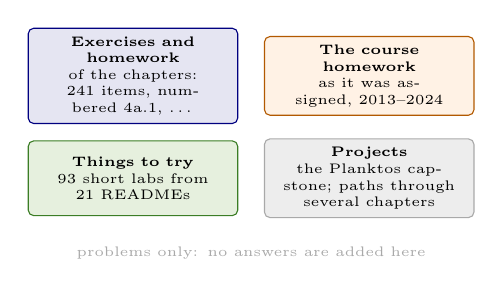
\begin{tikzpicture}[every node/.style={font=\tiny}, box/.style={draw, rounded corners=2pt, align=center, inner sep=3pt, text width=2.45cm, minimum height=0.95cm}]
  \node[box,draw=NavyBlue,fill=NavyBlue!10] (e) at (0,0) {\textbf{Exercises and homework}\\of the chapters: 241 items, numbered 4a.1, \ldots};
  \node[box,draw=orange!70!black,fill=orange!10] (c) at (3.0,0) {\textbf{The course homework}\\as it was assigned, 2013--2024};
  \node[box,draw=OliveGreen,fill=OliveGreen!10] (t) at (0,-1.3) {\textbf{Things to try}\\93 short labs from 21 READMEs};
  \node[box,draw=DarkGray,fill=LightGray!40] (p) at (3.0,-1.3) {\textbf{Projects}\\the Planktos capstone; paths through several chapters};
  \node[text=DarkGray,align=center,text width=5.4cm] at (1.5,-2.25) {problems only: no answers are added here};
\end{tikzpicture}}
\end{frame}

% 2
\begin{frame}{How to use the bank}
\label{fr:use}
\begin{columns}[T,onlytextwidth]
\begin{column}{0.52\textwidth}
\footnotesize
\begin{itemize}\setlength{\itemsep}{3pt}
  \item \al{Numbers:} \code{4d.3} is chapter 4d's third exercise, word for word as in the chapter; \code{6.E} a chapter's ``Extension'' and \code{4a.V} a homework variant, copied with their slide; \code{IB/11.2} the second ``Things to try'' item of example IB/11's README (\code{IBFE/06.1} for IBFE/06, \code{CIB/01.1} for ConstraintIB/01). Give them as assignments.
  \item \al{Slide numbers} in a copied slide (``slide 12'') are pages of that chapter's PDF, named in the slide's credit; the hand-written slides say ``slide 27 of chapter 9a''; other slide numbers (``the 2014 slide 10'', the lecture's ``slide 7'') are the old decks'.
  \item \al{The files} are in this repository's \code{examples/}; chapter 36 has one page per example.
  \item \al{Problems only:} no answers are added here. Slide \ref{fr:assign} lists what a student could find elsewhere before doing an exercise.
\end{itemize}
\end{column}
\begin{column}{0.45\textwidth}
\footnotesize
\begin{itemize}\setlength{\itemsep}{3pt}
  \item The bank, chapter by chapter: slides \ref{fr:index1}--\ref{fr:index2}.
  \item The course homework as it was assigned: slides \ref{fr:hw1}--\ref{fr:hw4}.
  \item The exercises, Part by Part: from slide \ref{fr:c4ax1}.
  \item Things to try, example by example: from slide \ref{fr:ttt1}.
  \item Projects: slides \ref{fr:proj1}--\ref{fr:proj2}.
\end{itemize}
\begin{punchbox}
\scriptsize Chapters 0.1--3 (front matter and setting up), 34 and Appendix B have no exercise slides: their checks are the runs themselves. The slides that quote course homework together with its answer (chapter 9a: 27; 16: 22--25; 18: 14, 18--20; 20: 16--17) are pointed to from slides \ref{fr:hw1}--\ref{fr:hw4}, not copied; chapter 35's exercise is its capstone (slide \ref{fr:proj1}).
\end{punchbox}
\end{column}
\end{columns}
\end{frame}

% 2b
\begin{frame}{Before you assign: where an exercise's outcome can already be read}
\label{fr:assign}
\footnotesize
\begin{itemize}\setlength{\itemsep}{3pt}
  \item \al{The copied Things to try} keep what their READMEs say, and some give the outcome of a chapter exercise: 8a.1 and IB/01.1; 9b.3 and IB/11.4; 10.2 and IB/09.3; 10.4 and IB/10.3; 12.2 and IB/08.2; 13.2--13.3 and IB/12.2--12.3; 14.3 and CIB/03.1; 17.4 and IBFE/01.2; 20.1 and IBFE/06.2; 21.1 and IBFE/08.1. Assign the exercise before the Things to try.
  \item \al{The chapters} print the answers to some course homework: chapter 9a's slide 27 (move and stretch), chapter 16's slides 22--25 (the two exercises and the 2021 lab, with the expected behaviour in their comments), chapter 18's slides 18--20 (the triangle homework), chapter 20's slides 16--17 (the travelling wave and its 2017 solutions), chapter 35's slides 47 and 49 (a complete capstone and its results). Chapter 5's ``Try it'' listings mark the stable and unstable runs.
  \item \al{The examples' READMEs} report what a run should give (their ``What you should see''); that is what a student's run is compared with, and many exercises ask for exactly that comparison.
\end{itemize}
\sourcecredit{The fact-check of this appendix (October 2026), which matched every exercise with the slides and READMEs that answer it.}
\end{frame}

\begin{frame}{The bank, chapter by chapter (1/2)}
\label{fr:index1}
\scriptsize
\renewcommand{\arraystretch}{1.0}
\begin{tabular}{@{}L{0.08\textwidth}L{0.55\textwidth}L{0.2\textwidth}L{0.08\textwidth}@{}}
\toprule
chapter & title & numbers & items\\
\midrule
4a & IB2d: introduction and file formats & 4a.1--4a.5, 4a.V & 5 + V\\
4b & The IB2d practical; VisIt for IB2d & 4b.1--4b.6 & 6\\
4c & IB2d: moving boundaries, your own example & 4c.1--4c.6, 4c.V & 6 + V\\
4d & IB2d: stability and convergence lab & 4d.1--4d.11 & 11\\
4e & IB2d: model gallery and muscles & 4e.1--4e.10 & 10\\
4f & IB2d: meshes from images & 4f.1--4f.6 & 6\\
5 & The IB method & 5.1--5.2 & 2\\
6 & Structure files & 6.1--6.3, 6.E & 3 + E\\
7 & Boundary conditions and the domain & 7.1--7.4, 7.E & 4 + E\\
8a & Changing physical parameters wisely & 8a.1--8a.4, 8a.E & 4 + E\\
8b & Non-dimensionalization & 8b.1--8b.4, 8b.E & 4 + E\\
9a & Target points and springs & 9a.1--9a.5, 9a.E & 5 + E\\
9b & Custom spring forces and active pumping & 9b.1--9b.5, 9b.E & 5 + E\\
10 & Resting curvature and beams & 10.1--10.5, 10.E & 5 + E\\
11 & Output and analysis of forces & 11.1--11.5, 11.E & 5 + E\\
12 & 3D simulations & 12.1--12.5, 12.E & 5 + E\\
13 & Adding mass & 13.1--13.5, 13.E & 5 + E\\
14 & Constraint IB & 14.1--14.5 & 5\\
15 & Tour of the upstream examples & 15.1--15.6 & 6\\
16 & What can go wrong & 16.1--16.5 & 5\\
\bottomrule
\end{tabular}
\end{frame}

\begin{frame}{The bank, chapter by chapter (2/2)}
\label{fr:index2}
\scriptsize
\renewcommand{\arraystretch}{1.0}
\begin{tabular}{@{}L{0.08\textwidth}L{0.55\textwidth}L{0.2\textwidth}L{0.08\textwidth}@{}}
\toprule
chapter & title & numbers & items\\
\midrule
17 & Getting started with IBFE & 17.1--17.6 & 6\\
18 & Creating meshes & 18.1--18.7 & 7\\
19 & PK1 stress functions and body forces & 19.1--19.7 & 7\\
20 & Fibre tension and active stress & 20.1--20.7 & 7\\
21 & Two or more meshes & 21.1--21.6 & 6\\
22 & 3D flow past objects & 22.1--22.8 & 8\\
23 & Walking through a main file & 23.1--23.6 & 6\\
24 & IBFE with advection--diffusion & 24.1--24.7 & 7\\
25 & Tour of the upstream IBFE examples & 25.1--25.9 & 9\\
26 & VisIt: getting started & 26.1--26.7 & 7\\
27 & VisIt in 3D & 27.1--27.7 & 7\\
28 & VisIt: Lagrangian and finite-element data & 28.1--28.8 & 8\\
29 & VisIt: data analysis & 29.1--29.7 & 7\\
30 & VisIt: movies & 30.1--30.8 & 8\\
31 & VisIt on the cluster & 31.1--31.7 & 7\\
32 & VisIt from Python & 32.1--32.7 & 7\\
33 & Converting data; MATLAB and Python & 33.1--33.8 & 8\\
36 & Catalogue of examples & 36.1--36.7 & 7\\
A & Appendix A: helper codes & A.1--A.5 & 5\\
\bottomrule
\end{tabular}
\end{frame}


% the course homework, as assigned
\begin{frame}{The course homework as it was assigned (1/4): the UA course, 2021--2024}
\label{fr:hw1}
\footnotesize
The University of Arizona course (MATH 481/581, Lectures 9--19, IB2d):
\begin{itemize}\setlength{\itemsep}{3pt}
  \item \al{Homework 4} (Lectures 9 and 11): your own rubber band in IB2d: make it 50\,\% smaller and deformed differently with your own generator, run it, and hand in two pictures, the initial state and the first dump after it, with the points, the velocity vectors and the vorticity. The 2021 variant (option 1): run an example related to your project instead and hand in the same two pictures. \emph{Now 4a.2--4a.3 (4a.1, 4a.4--4a.5 add to it), 4b.1 (the two pictures) and 4c.1.}
  \item \al{Homework 5} (Lecture 19, the stability lab): part 1, \code{stiff\_ode\_example} with $(0.2, 1)$, $(0.1, 1)$, $(0.01, 1)$; part 2, \code{heat\_equation} with $T = 100$ and $n = 3, 5, 10, 20$, then $n = 10$ and $T = 2, \ldots, 64$; part 3, the rubber band at $\Delta t = 1$ and at 1000 times the stiffness; part 4, the band refined from $32$ to $64$. \emph{Now 4d.1--4d.4.}
  \item \al{Homework 5's lab} (Lecture 19, slides 34--39, 2021): set the rubber band's \code{dt} to $1.0$ and \code{Tfinal} to $100$; put \code{dt} back and raise \code{kappa\_spring} from \code{2.0e3} to \code{2.0e6}; then raise \code{N} from 32 to 64 in the generator with \code{npts = ceil(2*(band\_length/L)*N)} and \code{Nx}, \code{Ny} in the input. \emph{Now 4d.3--4d.4; chapter 16 translates it to IBAMR (slides 24--25 of chapter 16).}
  \item \al{Homework 6}: share the geometry you will use for your project (a 3D object found or made for 3D printing or ANSYS, or an IB2d generator, with pseudo-code for its motion). \emph{Now 4d.10--4d.11.}
\end{itemize}
\sourcecredit{Chapters 4a, 4b, 4c, 4d and 16, which quote the lectures.}
\end{frame}

\begin{frame}{The course homework as it was assigned (2/4): the IBAMR course, 2013}
\label{fr:hw2}
\footnotesize
Homework 1 of the 2013 course (``Homework \#1, MATH 564'', due 19 February 2013), its IBAMR problems; the examples then ran on the lab's server or on UNC's clusters.
\begin{enumerate}\setlength{\itemsep}{2pt}
  \item The 2D moving bristles (formerly moving plates), with \code{END\_TIME = 0.05}: plot cycle 40000 with a colour map of the vorticity, the velocity vectors and the boundaries, and hand in a screenshot.
  \item Determine and justify a choice of the characteristic velocity and length scale for this simulation, and calculate the Reynolds number.
  \item Increase and decrease the Reynolds number by an order of magnitude; make the plots of problem 1 again.
  \item The multiple-boundaries example, with \code{END\_TIME = 0.1}: plot cycle 100000 the same way.
  \item Remove the target points from the lower 80\,\% of each plate, rerun, and plot cycle 100000 again.
\end{enumerate}
\emph{Today the bristles are IB/04 and the plates IB/07 (chapter 9a); the Reynolds number is chapter 8b's and the plots chapter 26's; related items: 8b.1, IB/04.2, 9a.2 and IB/07.4. The cycle numbers are those of the 2013 inputs. The homework's pencil-and-paper fluids problems belong to the theory series, \emph{Fluid Dynamics and IBM Theory}.}
\sourcecredit{The 2013 homework document (its answer key is not reproduced).}
\end{frame}

\begin{frame}{The course homework as it was assigned (3/4): the IBAMR courses, 2015--2020}
\label{fr:hw3}
\footnotesize
\begin{itemize}\setlength{\itemsep}{3pt}
  \item \al{Your own rubber band} (IBAMR Lecture 3, ``IBAMR associated files'': homework 2 of the 2018 course, and again in 2020): copy the rubber-band example and write your own generator, in any language, for the \code{.vertex} points and the \code{.spring} springs; make the band 50\,\% smaller and deform it initially in a different way; run it and look at it in VisIt. The 2018 version asked for two screenshots of the band oscillating; the 2020 version for the generator and the pictures in a shared folder. \emph{Now 6.1--6.3; the IB2d versions are 4a.2 and 4c.1.}
  \item \al{Stretching and shrinking plates} (2015--2016): in the moving-plates example, comment out where the plates are moved in \code{update\_target\_point\_positions} and remove the comment from \code{update\_springs}: one plate stretches and the other shrinks. Then the question of 2015--2020: ``Move and stretch? You do not want to move the boundaries with target points and stretch/shrink the plates at the same time. Why would this be problematic?'' \emph{Chapter 9a, slide 27 (``Stretching and shrinking plates (the 2015--2016 exercise)''), with IB/07; it also gives the answer. Now 9a.3.}
\end{itemize}
\vspace{1mm}
The homework slides of chapters 6--16 build on these courses' exercises and add new ones; each is in the bank under its chapter.
\sourcecredit{Chapters 6 and 9a, which quote the lectures.}
\end{frame}

\begin{frame}{The course homework as it was assigned (4/4): the IBFE series, 2014--2024}
\label{fr:hw4}
\footnotesize
\begin{itemize}\setlength{\itemsep}{3pt}
  \item \al{A travelling wave of tension} (IBFE tutorial on fibre tension, 2014, slide 11; 2020, slide 23): ``Take example 2 and apply tension as a sine wave that travels down the body. Note that you want to use something like \code{1.0/2.0* (1.0+sin((2.0*pi*(s(0)/body\_length + time)))} to not create negative tension. Squeeze the top and the bottom out of phase using the traveling sine wave (see example 3 for ideas)''. The expression has one more \code{(} than \code{)}; the intended tension is $T(\mathbf{s}, t) = \tfrac12\,T_{\max}\bigl(1 + \sin 2\pi(s_0/L + t)\bigr)$. \emph{Chapter 20, slide 16 (``The homework, and the tension that must not go negative''), which also gives the code. Now 20.1--20.2; IBFE/06.2--06.3 in the Things to try.}
  \item \al{Make your own mesh and move it} (2017--2024): in gmsh, a triangle with corners $(0.5, 0)$, $(0, 0)$ and $(0, 0.5)$ (``Remember you want to select these so they will fit in your domain''), with the prescribed element size at each point equal to the fine grid spacing ($0.0156$ at $\mathrm{NFINEST} = 128$); export it as MSH, version 2 ASCII; put it into the tethered-plate example in place of the plate (``In \code{main.C}, search for \code{IBFE\_Mesh2D\_128.mat}, replace with \code{triangle.msh}''), set \code{MFAC = 1.0} and \code{IB\_POINT\_DENSITY = 1.0} (``You may also need to change \code{DT} to something smaller''), and run it. \emph{Chapter 18, slides 14 and 18--20 (``The triangle of IBFE/05 (2)'', ``The GUI route (1)''--``(2)'', ``The homework's last two slides: what to change in the program and the input''); example IBFE/05. Now 18.1--18.2 and IBFE/05.1--05.3.}
\end{itemize}
\sourcecredit{Chapters 18 and 20, which quote the tutorials.}
\end{frame}

% ================= Part II, IB2d
% chapter 4a
% key: ex|4a|Exercise: your own rubber band (homework 4 of the UA course)
\begin{frame}{4a\,\textbullet\ IB2d: introduction and file formats (4a.1--4a.5)}
\label{fr:c4ax1}
\small
\begin{enumerate}
  \item[4a.1] Run \code{Rubberband\_with\_Springs} in MATLAB or Python as shipped. Note the wall time and the number of dumps. Open \code{lagsPts.0000.vtk} in a text editor and find the first point of the \code{.vertex} file in it.
  \item[4a.2] Copy the folder. In the generator, make the band 50\,\% smaller and deform it differently (stretched in $y$ instead of $x$, or a square, or a circle with a dent); keep $N$ so that $\Delta s \approx \Delta x/2$ along the new shape. Run the generator, run the checker of slide 52, then run \code{main2d}.
  \item[4a.3] Plot the structure at $t = 0$ and at the first dump after it, with the velocity vectors and the vorticity (matplotlib or MATLAB now, VisIt after chapter 4b), and write two sentences on what the band did.
  \item[4a.4] Change one flag: turn the springs into damped springs (write the \code{.d\_spring} file from the \code{.spring} one, add a column, switch the flags) and compare the half-width curve of slide 59.
  \item[4a.5] If you use the Python version, convert the MATLAB \code{NL\_Rubberband\_With\_Springs} example (nonlinear springs, $\alpha = 2$) to it: the files need the index shift of slide 35, \code{input2d} needs nothing.
\end{enumerate}
\al{4a.V} The 2021 variant of the homework (Lecture 11): run an example related to your project instead, and hand in the same two pictures.
\sourcecredit{Chapter 4a, slide ``Exercise: your own rubber band (homework 4 of the UA course)''. Slide numbers in it are pages of chapter 4a's PDF.}
\end{frame}

% chapter 4b
% key: ex|4b|Exercises
\begin{frame}{4b\,\textbullet\ The IB2d practical; VisIt for IB2d (4b.1--4b.6)}
\label{fr:c4bx1}
\small
\begin{enumerate}
  \item[4b.1] The practical's two: change the band so that it is stretched in $y$ instead of $x$ (``enough that you can see it''), and change the viscosity in \code{input2d} to put the band in a very viscous fluid. Plot the initial state and the first dump after it with the points, the vectors and the vorticity (homework 4 of Lecture 11), and say in two sentences how the viscous run differs.
  \item[4b.2] Save a VisIt session of the finished window; restore it with sources on the viscous run's folder.
  \item[4b.3] Make a 76-frame movie of the vorticity with fixed limits, as PNG frames joined by ffmpeg; note the file size against the wizard's MPEG.
  \item[4b.4] From \code{hier\_IB2d\_data}, plot the maximum of \code{fMag} against time for the springs band and for the damped-springs band of chapter 4a on the same axes.
  \item[4b.5] Run \code{HeartTube\_Muscle} and open it in VisIt: a Pseudocolor of \code{uMag} with the connected points; find the time of the strongest pinch from the \gui{MinMax} query over the states.
  \item[4b.6] Apply the one-line fix of slide 29 and run the pump; with chapter 33's reader, plot the mean $x$ of the tracers against time, unwrapping the jumps of tracers that cross the periodic edge, and read off the pumping speed.
\end{enumerate}
\sourcecredit{Chapter 4b, slide ``Exercises''. Slide numbers in it are pages of chapter 4b's PDF.}
\end{frame}

% chapter 4c
% key: ex|4c|Exercises
\begin{frame}{4c\,\textbullet\ IB2d: moving boundaries, your own example (4c.1--4c.3)}
\label{fr:c4cx1}
\small
\begin{enumerate}
  \item[4c.1] The course's homework: modify the rubber band so that it is 50\,\% smaller and deformed differently, with your own generator (Lectures 3 and 9); then drive it along a circle with an update function written in the second style (position as a function of time), and compare the band's centre with the prescribed path.
  \item[4c.2] On the full grid (MATLAB, or Python on a cluster), move the sawtooth's bottom row in antiphase (Lecture 3's line) and compare the flow rate through the middle with the one-row pump; then set the top row's amplitude so that its tips reach the bottom row's ($a = 2G$) and see what the occlusion does.
  \item[4c.3] Port the two-beam template to Python with the three fixes of slide 25: a 256-point beam each, the first quarter of each driven; run it at $128 \times 256$ and plot the flow rate between the beams.
\end{enumerate}
\sourcecredit{Chapter 4c, slide ``Exercises''. Slide numbers in it are pages of chapter 4c's PDF.}
\end{frame}

% chapter 4c
% key: ex|4c|Exercises (2)
\begin{frame}{4c\,\textbullet\ IB2d: moving boundaries, your own example (4c.4--4c.6)}
\label{fr:c4cx4}
\small
\begin{enumerate}
  
  \item[4c.4] Take the moving band and halve $\Delta t$: compare the band's centre at $t = 0.025$ between the two runs for the increment style, then rewrite the function in the second style and compare again.
  \item[4c.5] Draw two phases of a shape of your own (a bell, a fin, a chamber), write them as the pulsing heart's four-column file, and run it with the same function; then change the blend to $\frac12(1 - \cos 2\pi t/P)$ and compare the vorticity at the opening.
  \item[4c.6] Design an example of your own from the project ideas of Lecture 2 (a barb moving towards a circle, a heart tube that pumps, a leaf that vibrates in a flow) following slide 23; hand in the sketch, the generator, the function and the first two dumps.
\end{enumerate}
\al{4c.V} Lecture 11's homework 4, option 1: run an example related to your project instead.
\sourcecredit{Chapter 4c, slide ``Exercises (2)''. Slide numbers in it are pages of chapter 4c's PDF.}
\end{frame}

% chapter 4d
% key: ex|4d|Exercises
\begin{frame}{4d\,\textbullet\ IB2d: stability and convergence lab (4d.1--4d.6)}
\label{fr:c4dx1}
\small
\begin{enumerate}
  \item[4d.1] The course's homework 5, part 1: run \code{stiff\_ode\_example} with $(0.2, 1)$, $(0.1, 1)$, $(0.01, 1)$ and explain each plot with the factor $1 - 15\Delta t$; then add the trapezoidal step (slide 12) and repeat.
  \item[4d.2] Part 2: \code{heat\_equation} with $T = 100$ and $n = 3, 5, 10, 20$, then $n = 10$ and $T = 2, \ldots, 64$; tabulate $r$ and the maximum error; find the $T$ at which $n = 20$ beats $n = 10$, and explain it with slide 24.
  \item[4d.3] Part 3: the rubber band at $\Delta t = 1$ and at 1000 times the stiffness, in MATLAB or Python; quote the exact error line of your port.
  \item[4d.4] Part 4: refine $32 \to 64$ the course's way (same $\kappa$ in \code{generate\_mesh2d.m}, both files updated) and the chapter's way (\code{sweep.py grid2}); compare the time of the first $r_y$ minimum between the two and say which run is ``the same band''.
  \item[4d.5] Extend the map (slide 33) along a line $k = 2.5 \cdot 10^4$ at $64^2$ and $128^2$: does $\Delta t_{\max}$ halve with $\Delta x$?
  \item[4d.6] The 100-times-stiffer band fails by $t = 0.1$ at every $\Delta t$ on $32^2$ (before the first dump for $\Delta t \ge 10^{-3}$): run it at $64^2$ and $128^2$ with $\Delta t = 10^{-4}$ and report whether a finer grid takes it.
\end{enumerate}
\sourcecredit{Chapter 4d, slide ``Exercises''. Slide numbers in it are pages of chapter 4d's PDF.}
\end{frame}

% chapter 4d
% key: ex|4d|Exercises (2)
\begin{frame}{4d\,\textbullet\ IB2d: stability and convergence lab (4d.7--4d.9)}
\label{fr:c4dx7}
\small
\begin{enumerate}
  
  \item[4d.7] Measure the order in time of IB2d on the same band ($64^2$, four time steps), in Python or MATLAB (\code{analyze.py} reads the MATLAB dumps too), with the dumps' one-step lag removed (slide 42): compare states at the same step-corrected time, or compare the time of the first minimum of $r_y$ interpolated from the dumps, or use the fork branch's final dump, which is written at exactly $T_{\text{final}}$: first or second?
  \item[4d.8] Run the grid series one grid further ($512^2$, a cluster job: chapter 1) and add the row to the tables of slides 39 and 40.
  \item[4d.9] The volume error: plot the area inside the band against time for $32^2$ to $256^2$ and fit the loss at $t = 1$ to a power of $\Delta x$; then run the same band in IBAMR (chapter 5's rubber band, \code{examples/IB/01-rubber-band}) at the same resolutions and compare.
\end{enumerate}
\sourcecredit{Chapter 4d, slide ``Exercises (2)''. Slide numbers in it are pages of chapter 4d's PDF.}
\end{frame}

% chapter 4d
% key: ex|4d|Preparing the project geometry: the course's homework 6
\begin{frame}{4d\,\textbullet\ IB2d: stability and convergence lab (4d.10--4d.11)}
\label{fr:c4dx10}
\small
\al{The course's homework 6 (``you will share your geometry that you will use for your project''):}
\begin{itemize}
  \item[4d.10] 3D print or ANSYS: find a 3D object online (Thingiverse, GrabCAD) and explain what it is, or leave a note of anything you cannot find; create your own (SolidWorks, Autodesk Fusion); or mix: find an object and distort it. Share those objects.
  \item[4d.11] IB2d: geometries are created with a generator (\code{generate\_mesh}, chapter 4c); write code that gives the $x, y$ coordinates of the shape you want and submit it; if the object moves, give pseudo-code for how (the \code{update\_*} functions of chapter 4c).
\end{itemize}
\sourcecredit{Chapter 4d, slide ``Preparing the project geometry: the course's homework 6''; Lecture 19, slides 2 and 40.}
\end{frame}

% chapter 4e
% key: ex|4e|Exercises
\begin{frame}{4e\,\textbullet\ IB2d: model gallery and muscles (4e.1--4e.5)}
\label{fr:c4ex1}
\small
\begin{enumerate}
  \item[4e.1] Re-run \code{Gravity\_Cellular\_Race} with walls: a channel of target points around the three cylinders (as the MATLAB \code{Gravity\_vs\_Flow} race has, without its flow; the MATLAB \code{Gravity\_Cellular\_Race}, like the Python one, has none); repeat the momentum check of slide 14 and find the terminal speeds relative to the fluid.
  \item[4e.2] Give the porous band springs of non-zero resting length (\code{L} = the initial spacing): does it still collapse? Plot its area against time for three permeabilities and fit the rate.
  \item[4e.3] Change \code{User\_Defined\_Fiber\_Model} into a cubic spring ($F = k(|d| - L)^3$) and compare the band with the linear one; then into a spring that only pulls (no force when $|d| < L$).
  \item[4e.4] In \code{Concentration\_Diffusion}, set $\mu = 0.01$ and stir the box with an external force; check whether the total amount is still conserved (slide 24: the upwind advection does not conserve it in a moving fluid), and measure the mixing time.
  \item[4e.5] Give the heart tube's activation file a stored previous length, so that lengthening muscles get an eccentric branch (force above $F_{\max}$, which Hill's law, for shortening only, does not have; e.g.\ the $\alpha_p$ branch of slide 48) instead of the shortening one; compare the pinch and the flux.
\end{enumerate}
\sourcecredit{Chapter 4e, slide ``Exercises''. Slide numbers in it are pages of chapter 4e's PDF.}
\end{frame}

% chapter 4e
% key: ex|4e|Exercises (2)
\begin{frame}{4e\,\textbullet\ IB2d: model gallery and muscles (4e.6--4e.10)}
\label{fr:c4ex6}
\small
\begin{enumerate}
  
  \item[4e.6] Set the heart tube's \code{a} to $0.25\,F_{\max}$ (Hill's $a/P_0$) and run 20 periods; measure the mean flux at three sections, then vary the pulse speed (the \code{freq}) and find where the direction of pumping changes.
  \item[4e.7] Replace the heart tube's square pulse by the calcium model: each muscle stimulated for 5 ms when the wave passes, its $Caf$ integrated in the activation file; compare a 10 Hz train with a single wave.
  \item[4e.8] Show from the slide 42 formulas that a linear crossbridge spring $p = kx$ gives a linear force--velocity curve; plot it against the exponential spring's.
  \item[4e.9] With \code{calcium\_activation.py}, find the stimulus frequency at which the twitches fuse (the minimum of $Caf$ over a period reaches 90\,\% of its maximum) for three values of $k_4$; relate it to the twitch's half-decay time.
  \item[4e.10] Write the two-element model of slide 48 for an isometric muscle ($V = 0$) and integrate $P(t)$ for a twitch and for a tetanus.
\end{enumerate}
\sourcecredit{Chapter 4e, slide ``Exercises (2)''. Slide numbers in it are pages of chapter 4e's PDF.}
\end{frame}

% chapter 4f
% key: ex|4f|Exercises
\begin{frame}{4f\,\textbullet\ IB2d: meshes from images (4f.1--4f.6)}
\label{fr:c4fx1}
\small
\begin{enumerate}
  \item[4f.1] Trace a leaf, a fin or a wing of your own in Inkscape over a photograph; run \code{svg\_to\_vertex.py} at $64^2$, $128^2$ and $256^2$ and plot the points over the outline. How many points does the outline get at each grid?
  \item[4f.2] Run \code{svg\_to\_vertex.py --fit stretch} on the starfish in a $1 \times 0.25$ box and compare its aspect ratio with \code{--fit uniform}'s.
  \item[4f.3] Write the three-point Gauss rule and a subdividing version (split at $t = \frac12$ until two levels agree to $10^{-6}$); compare their errors on 1000 random cubics.
  \item[4f.4] Re-run the starfish channel with $k = 10^5$ and $10^6$ in the forcing (and $\Delta t$ halved if needed); plot the realised centre-line speed against the target. What $U_{\max}$ gives a peak of 1?
  \item[4f.5] Put three starfish in the channel (the paper's figure 10) by copying and translating the point set; compare the wake of the middle one with a single starfish.
  \item[4f.6] Give the starfish springs and beams between neighbours instead of targets (soft arms), keeping one target at its centre; what does the flow do to the arms? (IB2d's \code{Starfish} folder already gives its starfish springs, $10^7$ between neighbours and $10^5$ across, on top of the targets.)
\end{enumerate}
\sourcecredit{Chapter 4f, slide ``Exercises''.}
\end{frame}

% ================= Part III, IBAMR
% chapter 5
% key: ex|5|Try it: the stiff equation
\begin{frame}[fragile]{5\,\textbullet\ The IB method (5.1)}
\label{fr:c5x1}
\al{5.1}
\begin{columns}[T,onlytextwidth]
\begin{column}{0.5\textwidth}
In MATLAB or Octave, from \code{examples/support/matlab-exercises}:
\begin{lstlisting}[style=matlab]
stiff_ode_example(0.2, 1)    % unstable
stiff_ode_example(0.1, 1)    % stable, oscillates
stiff_ode_example(0.01, 1)   % smooth
\end{lstlisting}
In Python (the same plots, saved as \code{stiff\_ode\_example.png}; add \code{--show} for a window):
\begin{lstlisting}[style=shell]
python3 stiff_ode_example.py 0.2 1
python3 stiff_ode_example.py 0.1 1
python3 stiff_ode_example.py 0.01 1
\end{lstlisting}
\end{column}
\begin{column}{0.48\textwidth}
\begin{itemize}
  \item The arguments are the time step and the final time.
  \item Find the largest stable step by halving and doubling; then check the claim $\Delta t \le 2/15$ with $\Delta t = 0.13$ and $0.14$.
  \item Change $-15$ to $-150$ in the script. What happens to the stable step?
\end{itemize}
\begin{punchbox}
\small The scripts are the course's, with two bugs fixed: the MATLAB version allocated \code{zeros(N)} (an $N\times N$ matrix) instead of a vector and stopped one step before \code{tfinal}. The Python version writes the same numbers (Appendix A).
\end{punchbox}
\end{column}
\end{columns}
\sourcecredit{Chapter 5, slide ``Try it: the stiff equation''.}
\end{frame}

% chapter 5
% key: ex|5|Try it: the heat equation
\begin{frame}[fragile]{5\,\textbullet\ The IB method (5.2)}
\label{fr:c5x2}
\footnotesize
\al{5.2}
\begin{columns}[T,onlytextwidth]
\begin{column}{0.5\textwidth}
\begin{lstlisting}[style=matlab,basicstyle=\ttfamily\tiny\color{BlackGray}]
heat_equation(n, T)   % n interior points, T steps to t = 0.1
heat_equation(3, 100), heat_equation(5, 100)
heat_equation(10, 100), heat_equation(20, 100)  % space
heat_equation(19, 25), heat_equation(19, 50)    % unstable
heat_equation(19, 100), heat_equation(19, 200)  % stable
\end{lstlisting}
\begin{lstlisting}[style=shell,basicstyle=\ttfamily\tiny\color{BlackGray}]
python3 heat_equation.py 19 100   # dx = 0.05, r = 0.4
python3 heat_equation.py 19 50    # r = 0.8: blows up
python3 heat_equation.py 19 70    # r = 0.57: not yet visible
\end{lstlisting}
\end{column}
\begin{column}{0.48\textwidth}
\scriptsize
\begin{itemize}
  \item The plot shows the numerical and the exact solution at $t = 0.1$; the Python version prints the largest error, writes $\Delta x$, $\Delta t$ and $r$ on the plot and saves \code{heat\_equation.png}.
  \item The 2018 lecture used $n = 10$ with $T = 2, 4, 8, 16, 32, 64$. With so few points the unstable runs (any $T < 25$) have not yet grown visibly by $t = 0.1$, and the solutions look merely wrong; $n = 19$ with $T = 25$ and $50$ shows the real blow-up.
  \item The course's \code{heat\_equation.m} had a header that said $\sin 3\pi x$ while the code used $\sin 2\pi x$, and writes an EPS file on every call (\code{print -deps Example4\_1.eps}, left as it was: chapter 4d); the header is fixed, and the Python version gives the same numbers in the stable cases (checked with Octave; in the unstable ones the round-off that starts the blow-up differs from program to program, Appendix A).
\end{itemize}
\end{column}
\end{columns}
\sourcecredit{Chapter 5, slide ``Try it: the heat equation''.}
\end{frame}

% chapter 6
% key: ex|6|Homework: your own rubber band
\begin{frame}{6\,\textbullet\ Structure files (6.1--6.3)}
\label{fr:c6x1}
\begin{columns}[T,onlytextwidth]
\begin{column}{0.55\textwidth}
From the 2018 and 2020 courses:
\begin{enumerate}
  \item[6.1] Copy IB/01 and write your own generator, in any language, that puts down the \code{.vertex} points and the \code{.spring} springs of a rubber band.
  \item[6.2] Make the band \al{50\% smaller} and deform it initially in a different way (an ellipse the other way, a square, a band with a dent).
  \item[6.3] Run it and look at it in VisIt. The 2018 version asked for two screenshots of the band oscillating; the 2020 version for the generator and the pictures in a shared folder.
\end{enumerate}
\end{column}
\begin{column}{0.43\textwidth}
\begin{punchbox}
\small What to check in your files before running: the count equals the number of lines minus one; the indices run from 0; the ring is closed; the spacing is about $\Delta x/2$; the stiffness in the file is $K/\Delta s$ for the $K$ you chose. Then a short run and the log's ``read N'' lines.
\end{punchbox}
\vspace{2mm}
\small \al{6.E} Extension: add a \code{.beam} file to the band (IB/03's generator shows the loop) and watch the dent smooth out faster.
\end{column}
\end{columns}
\sourcecredit{Chapter 6, slide ``Homework: your own rubber band''.}
\end{frame}

% chapter 7
% key: ex|7|Homework
\begin{frame}{7\,\textbullet\ Boundary conditions and the domain (7.1--7.4)}
\label{fr:c7x1}
\begin{columns}[T,onlytextwidth]
\begin{column}{0.55\textwidth}
\footnotesize From the 2015--2020 courses and the READMEs:
\begin{enumerate}
  \item[7.1] IB/03: make the top and bottom walls stick (\code{gcoef\_function\_2} and \code{\_3} of the $x$-block to \code{"0.0"}) and compare the wake; then bring the flow in from the top instead of the left (which blocks change?).
  \item[7.2] IB/02: double \code{f}, halve \code{d}, and make the flow reverse. Describe the profile at a peak and at a zero crossing.
  \item[7.3] IB/03: put the leaf in a $2L \times L$ box with the leaf a quarter of the way in. Write the new \code{N}, \code{domain\_boxes}, \code{x\_lo}, \code{x\_up} and patch sizes before you run; check \code{DX} is unchanged.
  \item[7.4] IB/03: make the outlet open (traction, $g = 0$ on both components) with \code{NORMALIZE\_PRESSURE = FALSE}, and compare the wake near the outlet with the prescribed-outlet run.
\end{enumerate}
\end{column}
\begin{column}{0.43\textwidth}
\begin{punchbox}
\small What to hand in (the 2018--2020 pattern): the edited blocks, one VisIt frame per case with the boundary velocity visible, and two sentences on what changed. For item 3, also the arithmetic of slide 56.
\end{punchbox}
\vspace{2mm}
\small \al{7.E} Extension: in IB/08, set \code{SHEAR\_START = 1} and compare the force on the fibre at $t = 0.2$ s with the ramped run (the README has both numbers).
\end{column}
\end{columns}
\sourcecredit{Chapter 7, slide ``Homework''. Slide numbers in it are pages of chapter 7's PDF.}
\end{frame}

% chapter 8a
% key: ex|8a|Homework
\begin{frame}{8a\,\textbullet\ Changing physical parameters wisely (8a.1--8a.4)}
\label{fr:c8ax1}
\begin{columns}[T,onlytextwidth]
\begin{column}{0.6\textwidth}
\footnotesize From the 2015--2018 courses and the READMEs:
\begin{enumerate}
  \item[8a.1] IB/01: run the viscosity sweep (\code{MU} = 100, 10, 1), plot the band's half-width and half-height against time, and measure the swing period at \code{MU = 1}. Then find the viscosity at which the band is critically damped (no overshoot, fastest approach).
  \item[8a.2] IB/03: estimate the spring and beam stiffness of the leaf from slides 20 and 22, compare with the generator's values, and run the leaf at $k'_{\mathrm{beam}} = 10$. Report the tip angle.
  \item[8a.3] IB/03: double \code{V}. Before running, write down what changes (Re, forces, \code{DT}, \code{END\_TIME}); after running, say which of your predictions held.
  \item[8a.4] ``Imagine what this thing would be in reality'': pick one example and write its parameters as a real object with units (a jellyfish, a leaf in a stream, a glycocalyx fibre); then compute its Reynolds number and say whether the example's choice is realistic.
\end{enumerate}
\end{column}
\begin{column}{0.38\textwidth}
\begin{punchbox}
\footnotesize What to hand in: the edited lines (input file or generator), the one number you compared (slide 29), and one picture per run. For item 1, the plot; for item 2, the arithmetic.
\end{punchbox}
\vspace{1mm}
\footnotesize \al{8a.E} Extension: IB/08 with \code{RE = 1} through the viscosity option, compared with the shipped $\mu = 40$ run (the README has the force at $t = 0.2$ s for the shipped run).
\end{column}
\end{columns}
\sourcecredit{Chapter 8a, slide ``Homework''. Slide numbers in it are pages of chapter 8a's PDF.}
\end{frame}

% chapter 8b
% key: ex|8b|Homework
\begin{frame}{8b\,\textbullet\ Non-dimensionalization (8b.1--8b.4)}
\label{fr:c8bx1}
\begin{columns}[T,onlytextwidth]
\begin{column}{0.55\textwidth}
\footnotesize From the 2015--2018 courses and this chapter:
\begin{enumerate}
  \item[8b.1] Compute every dimensionless number of slide 29 for one example of your choice, stating $U$ and $L$. Compare with slide 30 and explain any difference.
  \item[8b.2] Convert a real organism to a simulation: pick an animal or organ with published size, speed and frequency, compute $\mathrm{Re}$, $\mathrm{St}$ (and $\alpha$ or $\mathrm{Pe}$ if relevant), and write the unit-scale input constants (\code{MU}, the frequency, \code{END\_TIME}) and the SI ones.
  \item[8b.3] IB/03 in unit scales: set $\rho = 1$, $\ell = 1$, $U = 1$, \code{MU = 1/2.5}, $k_{\mathrm{beam}} = 0.5$, $K = 30$ (regenerate the structure for a $10 \times 10$ box) and compare the tip deflection over length and $C_D$ with the SI run. They should agree.
  \item[8b.4] From the leaf's \code{integral\{F\}}, compute $C_D(t)$ (slide 20) and $F/(\mu U)$; say which one is nearly constant after $t' = 1$ and why.
\end{enumerate}
\end{column}
\begin{column}{0.43\textwidth}
\begin{punchbox}
\footnotesize What to hand in: a table of groups with the scales named, the input lines you changed, and one plot with dimensionless axes. For item 3, the two runs' numbers side by side.
\end{punchbox}
\vspace{1mm}
\footnotesize \al{8b.E} Extension: the growing fibre (IB/06) with the 2018 exercise's oscillating rest length, $0.00049\sin(2\pi t)$ per spring: predict its $\mathrm{St}_L$ before running, then measure the fibre's end-to-end length against time.
\end{column}
\end{columns}
\sourcecredit{Chapter 8b, slide ``Homework''. Slide numbers in it are pages of chapter 8b's PDF.}
\end{frame}

% chapter 9a
% key: ex|9a|Homework
\begin{frame}{9a\,\textbullet\ Target points and springs (9a.1--9a.5)}
\label{fr:c9ax1}
\begin{columns}[T,onlytextwidth]
\begin{column}{0.55\textwidth}
\scriptsize From the 2015--2020 courses and the READMEs:
\begin{enumerate}
  \item[9a.1] IB/04: make the row move sideways instead of up, and change \code{V} or \code{time\_to\_acc}; predict the lag from $\kappa$ and \code{integral\{F\}} before you measure it.
  \item[9a.2] IB/07: move only one plate; then tether only the middle point of each plate and watch them bend as they are dragged.
  \item[9a.3] IB/07: the stretch-and-shrink exercise with the corrected code; stop before the right plate's rest length reaches zero, and explain why ``move and stretch'' at once is a bad idea.
  \item[9a.4] IB/06: make the rest length oscillate, \code{A*sin(2*PI*f*t)*dt} per spring, with the 2018 numbers ($A = 0.00049$, $f = 1$ Hz); then halve \code{growth\_rate} in the original and report when the fibre buckles.
  \item[9a.5] Write a function that moves a structure between two drawn states (slide 30) and drive IB/03's leaf with it instead of the stream.
\end{enumerate}
\end{column}
\begin{column}{0.43\textwidth}
\begin{punchbox}
\scriptsize What to hand in (the 2018--2020 pattern): the changed lines of the update function, the \code{CMakeLists.txt} line, one VisIt frame per case, and the check of slide 34 that shows the motion was followed.
\end{punchbox}
\scriptsize \al{9a.E} Extension: move \code{V} and \code{time\_to\_acc} into the input file (slide 32) and run a job array over three speeds (chapter 8a).
\end{column}
\end{columns}
\sourcecredit{Chapter 9a, slide ``Homework''. Slide numbers in it are pages of chapter 9a's PDF.}
\end{frame}

% chapter 9b
% key: ex|9b|Homework
\begin{frame}{9b\,\textbullet\ Custom spring forces and active pumping (9b.1--9b.5)}
\label{fr:c9bx1}
\begin{columns}[T,onlytextwidth]
\begin{column}{0.6\textwidth}
\footnotesize From the 2013--2015 courses and this chapter:
\begin{enumerate}
  \item[9b.1] IB/11: run \code{TARGET\_VP} and \code{FORCE\_VP}, and find the $F_{\mathrm{mag}}$ at which the applied force gives the same squeeze as the targets. Compare the net flow per period (chapter 29) and the markers' drift.
  \item[9b.2] IB/11: halve $\mathrm{Wo}$ (the viscosity doubles) and halve the frequency, one at a time; say which changes the net flow per period more, which the markers' drift, and why (chapter 8b).
  \item[9b.3] Move the actuator to the middle of the elastic section (\code{Ca} in the generator). What happens to the net flow, and what does that say about valveless pumping?
  \item[9b.4] Write a cable (tension-only) law, register it under index 3, and give it to the springs of IB/01's rubber band. What does the band do when it is compressed?
  \item[9b.5] Write a muscle law with an active tension that the update function raises and lowers at 1 Hz on half of IB/06's fibre.
\end{enumerate}
\end{column}
\begin{column}{0.38\textwidth}
\begin{punchbox}
\scriptsize What to hand in: the force function and its registration line, the generator loop that writes the index, the \code{integral\{F\}} or marker check that shows the force acts, and one VisIt frame per run.
\end{punchbox}
\scriptsize \al{9b.E} Extension: compute $C_{\mathrm{pump}}$ (slide 30) for the two suction modes from the \code{X.*} and \code{F.*} files.
\end{column}
\end{columns}
\sourcecredit{Chapter 9b, slide ``Homework''. Slide numbers in it are pages of chapter 9b's PDF.}
\end{frame}

% chapter 10
% key: ex|10|Homework
\begin{frame}{10\,\textbullet\ Resting curvature and beams (10.1--10.5)}
\label{fr:c10x1}
\begin{columns}[T,onlytextwidth]
\begin{column}{0.56\textwidth}
\scriptsize From the 2013 course and this chapter:
\begin{enumerate}
  \item[10.1] IB/09: make the beam curl into a half circle instead of a quarter (change $\varphi_i$'s range and $R_{\mathrm{final}}$), and into a quarter circle the other way (the sign of $C_2$).
  \item[10.2] IB/09: give the beam the quarter circle's curvature in the \code{.beam} file from the start (the worksheet's recipe) and no update function. How long does it take to reach its shape, and how does that compare with the ramp?
  \item[10.3] IB/10: change $t_0$ to $0.3$ (a fast contraction, slow expansion) and compare the distance travelled per pulse; then $\beta_m = 0.3$ (a weaker contraction).
  \item[10.4] IB/10: double $\mu$ (halve the Reynolds number) and say what happens to the swimming speed; Herschlag and Miller 2011 is the reference.
  \item[10.5] Write the invariant angle form of the bending energy as a chapter 9b force strategy, and show that a rotated IB/09 beam curls the same way with it.
\end{enumerate}
\end{column}
\begin{column}{0.42\textwidth}
\begin{punchbox}
\scriptsize What to hand in: the \code{.beam} lines or the update function's curvature lines you changed, the generator loop, the step you had to use, and one VisIt frame per run with the shape and the vorticity.
\end{punchbox}
\scriptsize \al{10.E} Extension: compute the bending energy $E_b$ of IB/09 from the \code{X.*} files (chapter 11) and plot it against time; it should peak while the curvature is still changing.
\end{column}
\end{columns}
\sourcecredit{Chapter 10, slide ``Homework''.}
\end{frame}

% chapter 11
% key: ex|11|Homework
\begin{frame}{11\,\textbullet\ Output and analysis of forces (11.1--11.5)}
\label{fr:c11x1}
\begin{columns}[T,onlytextwidth]
\begin{column}{0.56\textwidth}
\scriptsize From the 2012--2020 courses and this chapter:
\begin{enumerate}
  \item[11.1] IB/03: run the course's 20 s (\code{END\_TIME = 20.0}) and plot $C_D$ to the plateau; compare with the 2013 figure's $1.6$. Then halve $\mu$ and say what happens to the plateau and to the ripple.
  \item[11.2] IB/07: the force on each plate against time from the \code{F} files (chapter 9a's README table), with the gap from the \code{X} files on the same axes.
  \item[11.3] IB/11: the work done by the actuator over the second period and the pump coefficient (chapter 9b), for the target-point and the applied-force modes.
  \item[11.4] IB/10: the bell's vertical force (the sum over the bell, which should be zero) and the apex's velocity from differences of positions; is the jellyfish accelerating during contraction or expansion?
  \item[11.5] Write the energy of IB/09's beam from the \code{X} files and the stiffnesses, and plot it against time.
\end{enumerate}
\end{column}
\begin{column}{0.43\textwidth}
\begin{punchbox}
\scriptsize What to hand in: the reader you used, the normalization (with $\rho$, $U$, $L$ and the convention), the raw and the filtered curve on one plot, and one sentence on the sign of each force.
\end{punchbox}
\scriptsize \al{11.E} Extension: rerun IB/03 with \code{-stokes\_ksp\_rtol 1e-12} and overlay the two raw $C_D$ curves.
\end{column}
\end{columns}
\sourcecredit{Chapter 11, slide ``Homework''.}
\end{frame}

% chapter 12
% key: ex|12|Homework
\begin{frame}{12\,\textbullet\ 3D simulations (12.1--12.5)}
\label{fr:c12x1}
\begin{columns}[T,onlytextwidth]
\begin{column}{0.56\textwidth}
\footnotesize From the 2012--2016 courses and this chapter:
\begin{enumerate}
  \item[12.1] IB/08: run the default $0.2$ s, then \code{SHEAR\_START = 1}, and compare the force on the fiber (chapter 11, \code{ndim = 3}) at the end of each.
  \item[12.2] IB/08: drag the fiber instead of the lid (\code{TARGET\_VELOCITY}), with the lid at rest; is the force the same?
  \item[12.3] Build the 2016 sheet with slide 11's recipe ($0.1$ m square, $\Delta s = \Delta x/2$ at $\Delta x = 1/256$ m), tether its centreline, put it in IB/08's box with a stream in $x$ (\code{periodic\_dimension = 0, 1, 0}), and run $0.5$ s. Report the number of points, cells and the time per step.
  \item[12.4] Add diagonal springs to the sheet and compare the shape at $0.5$ s.
  \item[12.5] IBFE/10: halve the plate's shear modulus and compare the bending (chapter 22).
\end{enumerate}
\end{column}
\begin{column}{0.43\textwidth}
\begin{punchbox}
\scriptsize What to hand in: the \code{input3d} blocks you changed, the generator loop, the point and cell counts, the time per step on the cores you used, and one VisIt image with a slice and the structure.
\end{punchbox}
\scriptsize \al{12.E} Extension: the two wings of the 2012 model, translated apart in 3D (IB/07's update function with \code{X\_target[0]}), on a coarse grid.
\end{column}
\end{columns}
\sourcecredit{Chapter 12, slide ``Homework''. Slide numbers in it are pages of chapter 12's PDF.}
\end{frame}

% chapter 13
% key: ex|13|Homework
\begin{frame}{13\,\textbullet\ Adding mass (13.1--13.5)}
\label{fr:c13x1}
\begin{columns}[T,onlytextwidth]
\begin{column}{0.56\textwidth}
\scriptsize From the 2020 course and this chapter:
\begin{enumerate}
  \item[13.1] IB/12: double the spider's mass and halve it; plot the three falls on one axes (chapter 11) and compare the terminal speeds with $m g$ against the drag.
  \item[13.2] IB/12: lengthen the dragline to $0.2$ m (the generator's \code{drag\_length}) and shorten it to $0.05$ m; which falls slower?
  \item[13.3] IB/12: raise the penalty stiffness to $200$ and lower it to $2$; measure $|\mathbf{Y} - \mathbf{X}|$ from the force on the mass point (the penalty force is $K(\mathbf{Y} - \mathbf{X})$), and find the step at which $200$ aborts.
  \item[13.4] Put the spider in a uniform cross-wind (chapter 7's boundary conditions, a ramped \code{V}) as the 2020 study's second case, and in a shear flow as its third.
  \item[13.5] Give IB/01's rubber band mass at every point (a \code{.mass} line each, the total mass of a $1$ mm-thick rubber ring per unit depth) and gravity; does it sink, and does it keep its shape?
\end{enumerate}
\end{column}
\begin{column}{0.43\textwidth}
\begin{punchbox}
\scriptsize What to hand in: the \code{.mass} lines, the input block, the step you used and the stability estimate, the height-against-time plot, and one VisIt frame with vorticity.
\end{punchbox}
\scriptsize \al{13.E} Extension: compare IB/12 with a constraint-IB rigid body of the same mass (chapter 14).
\end{column}
\end{columns}
\sourcecredit{Chapter 13, slide ``Homework''.}
\end{frame}

% chapter 14
% key: ex|14|Homework
\begin{frame}{14\,\textbullet\ Constraint IB (14.1--14.5)}
\label{fr:c14x1}
\footnotesize
\begin{enumerate}
  \item[14.1] ConstraintIB/01: do the lecture's exercise (slide 7, ``Alter the kinematics to make the cylinder go up and down''): write \code{[0][1][k]} instead of \code{[0][0][k]} and compare the $y$ force file with the $x$ one of the shipped run. Then tow it (\code{U\_infinity = 0}, \code{prescribed\_trans\_velocity = 1}) and read the drag coefficient $C_D = 2F/(\rho U^2 D)$ from the force file after it settles (chapter 11).
  \item[14.2] ConstraintIB/02: push the disc off centre (\code{XCOM = 0.2}) so that the impulse has a moment; read the angular velocity file. Then repeat with \code{needs\_divfree\_projection = FALSE} and say what changed in the momentum file.
  \item[14.3] ConstraintIB/03: halve the amplitude ($0.125 \to 0.0625$ in all three expressions) and run two beats; compare the swimming speed. Then switch \code{body\_is\_maneuvering = TRUE} and watch where the eel goes.
  \item[14.4] Write a kinematics class of your own: a disc that rolls (prescribed angular velocity, zero translation) by filling \code{d\_current\_kinematics\_vel} with $\boldsymbol{\Omega}\times\mathbf{R}$ about the centre of mass, which \code{setKinematicsVelocity} receives. Start from \code{OscillatingCylinderKinematics}.
  \item[14.5] Add a second structure: two discs, each with its own kinematics object and sub-block, \code{num\_structures = 2}; the force files get a \code{\_struct\_no\_1}.
\end{enumerate}
\sourcecredit{Chapter 14, slide ``Homework''.}
\end{frame}

% chapter 15
% key: ex|15|Homework
\begin{frame}{15\,\textbullet\ Tour of the upstream examples (15.1--15.6)}
\label{fr:c15x1}
\footnotesize
\begin{enumerate}
  \item[15.1] Build and run \code{IB/explicit/ex1} with \code{input2d}, then with \code{input2d.shell} and \code{input2d.shell\_circum\_fibers}; describe in one sentence each how the three bands differ in VisIt (chapter 26).
  \item[15.2] Run \code{IB/explicit/ex0}, which has no \code{.vertex} file, and find in \code{example.cpp} the function that \code{IBRedundantInitializer} calls to make the points; change the number of points and the radius.
  \item[15.3] Run \code{IB/explicit/ex5} for $200$ steps and watch the free points; then set \code{kT = 0} and say what happens to them, and why the lecture's description was wrong.
  \item[15.4] \code{navier\_stokes/ex2}: run the cavity for $100$ steps, then for $5{,}000$, and compare the centreline velocity with Ghia's values using the shipped \code{analyzer.m} (chapter 11 for the MATLAB side).
  \item[15.5] \code{adv\_diff/ex0}: run \code{converg2d} (read it first; it runs the example at several resolutions) and report the order of accuracy you get (chapter 16).
  \item[15.6] Pick the example nearest your own problem from slide 40, run it as shipped for two minutes, and write down what you would change first.
\end{enumerate}
\sourcecredit{Chapter 15, slide ``Homework''. Slide numbers in it are pages of chapter 15's PDF.}
\end{frame}

% chapter 16
% key: ex|16|Homework
\begin{frame}{16\,\textbullet\ What can go wrong (16.1--16.5)}
\label{fr:c16x1}
\footnotesize
\begin{enumerate}
  \item[16.1] IB/01: raise \code{DT} until the run aborts, then set \code{warn\_on\_dt\_change = TRUE} and \code{error\_on\_dt\_change = FALSE} and run again; plot \code{dt} from the log against time and say what the integrator did instead of stopping.
  \item[16.2] Run the two Python exercises of slides 22--23 at the lecture's parameters and at one more of your own each; write the stability condition you observed as an inequality.
  \item[16.3] Repeat the convergence study of slides 26--27 on IB/03 (chapter 8a's tethered beam) with the drag coefficient of chapter 11 as the number: three grids, one order.
  \item[16.4] Take the upstream cylinder of chapter 15 (\code{IB/explicit/ex2}) and set \code{vorticity\_rel\_thresh} to $0.5$, $0.25$ and $0.1$; count the finest-level cells in the log at $t = 20$ s and compare the wake in VisIt.
  \item[16.5] Make a run fail on purpose in three different ways (a key in the wrong block, a point outside the box, a stiffness ten times too high) and write down, for each, the first line of the log that gave it away.
\end{enumerate}
\sourcecredit{Chapter 16, slide ``Homework''. Slide numbers in it are pages of chapter 16's PDF.}
\end{frame}

% ================= Part IV, IBFE
% chapter 17
% key: ex|17|Exercises
\begin{frame}{17\,\textbullet\ Getting started with IBFE (17.1--17.6)}
\label{fr:c17x1}
\footnotesize
\begin{enumerate}
  \item[17.1] Translate the plate to the left at $0.3$ for one second (the 2014 slide 10), then release it. Where is its centre at $t = 2$? Compare with FULL's drift after release.
  \item[17.2] Add the sinusoidal body force of slide 25 (a new \code{MOTION = "SHAKE"} case, with the amplitude and frequency in the input) and run it for four periods, once on the ends as the 2016 code does and once on the middle half as the 2014 slide says. Which part of the plate moves most, and why is it not the forced part alone?
  \item[17.3] Repeat FULL with \code{KAPPA\_S = 1e4} and \code{1e2}. At which stiffness does the plate stop following the target, and what does the vorticity look like then?
  \item[17.4] Repeat HALF with \code{SHEAR\_MODULUS = 1} and watch the run stop. Read chapter 16's slide on \code{Time step size change encountered}, then find the largest \code{DT} that reaches $t = 4$.
  \item[17.5] Make the same plate in gmsh (chapter 18), run FULL with \code{MESH\_FILENAME} set to it, and compare the centre positions of slide 43. Then halve the element size and compare again.
  \item[17.6] Put a pressure load of slide 30 on the plate (no tether: \code{MOTION = "FULL"} with \code{KAPPA\_S = 0}) and explain what a uniform pressure on a closed boundary does to a nearly incompressible body.
\end{enumerate}
\sourcecredit{Chapter 17, slide ``Exercises''. Slide numbers in it are pages of chapter 17's PDF.}
\end{frame}

% chapter 18
% key: ex|18|Exercises
\begin{frame}{18\,\textbullet\ Creating meshes (18.1--18.7)}
\label{fr:c18x1}
\footnotesize
\begin{enumerate}
  \item[18.1] Make the IBFE/01 plate ($1.0\times0.0312$) in gmsh with \code{lc = 0.03}, export MSH 2.2, and run \code{MOTION = "FULL"} with it. Compare the centre positions with chapter 17's table; then halve \code{lc} and compare again.
  \item[18.2] Take \code{triangle.geo}, make the curve loop clockwise, mesh, and run IBFE/05 until it stops. Fix the file three ways (the loop, \code{ReverseMesh}, \code{fix\_orientation.py}) and check that all three meshes are the same.
  \item[18.3] Write the plate-with-a-hole \code{.poly} of slide 31, mesh it with \code{triangle -pqa0.0005}, convert the \code{.node}/\code{.ele} pair to MSH 2.2 with a script of your own, and run it in IBFE/01's program. What does the hole do to the FULL motion?
  \item[18.4] Finish Battista's tube: add the surface loop, volume and physical volume to the \code{.geo} he built, mesh it in 3D, and read it with the checker of slide 39. How many tetrahedra at \code{ds = L/100}?
  \item[18.5] Run \code{tube.geo} at the three densities $6/5/24$, $8/10/60$ and the original $15/20/200$; tabulate nodes, hexahedra, file size and the time gmsh takes. Which would you use at $\mathrm{DX} = 1/16$?
  \item[18.6] Rebuild IBFE/10's plate ($0.125\times2\times2$, about $3\,\mathrm{DX}$ elements) from a \code{.geo} of your own by extruding a square, and compare the node count with \code{plate2.msh}'s $3{,}386$.
  \item[18.7] Build the same plate inside the program with \code{build\_cube} and \code{MFAC = 3}, run both for $0.5$ s, and compare the tether force lines of the two runs.
\end{enumerate}
\sourcecredit{Chapter 18, slide ``Exercises''. Slide numbers in it are pages of chapter 18's PDF.}
\end{frame}

% chapter 19
% key: ex|19|Exercises
\begin{frame}{19\,\textbullet\ PK1 stress functions and body forces (19.1--19.7)}
\label{fr:c19x1}
\footnotesize
\begin{enumerate}
  \item[19.1] Remove the dilational function from IBFE/01 (comment out its \code{registerPK1StressFunction}) and run \code{FULL} to $t = 0.5$. Measure the plate's length from \code{output.ex2} and explain the sign of the change from slide 9.
  \item[19.2] Replace the neo-Hookean pair by the compressible law of IBFE/10 with $\beta = 10\mu$ and $\beta = 100\mu$ (\code{MOTION = "HALF"}). Print $J$'s range every 50 steps as IBFE/10 does. Which $\beta$ is worth its time step?
  \item[19.3] Write the St.\ Venant--Kirchhoff law of ex7 for the plate with $\lambda = \mu$ and compare the tilt at $t = 1$ with the neo-Hookean $39^\circ$.
  \item[19.4] Make the plate's left half ten times stiffer than its right (test \code{s(0)} in both stress functions), run \code{HALF}, and explain the tilt you get from slide 16.
  \item[19.5] Add gravity (slide 21) with $\rho_s - \rho_f = 0.2$ and $g = 1$ to \code{MOTION = "FULL"} after the release; where is the centre at $t = 4$ compared with chapter 17's $-0.936$?
  \item[19.6] Make the tether of IBFE/01 a damped one as in ex5 ($\eta_s = 10^3$): register the velocity system, read it from \code{var\_data}, and compare the overshoot at $t = 1$ with slide 26's $0.507$.
  \item[19.7] Turn the plate's tether into a surface force on its long edges only (ex8's \code{side} test). Does the plate still follow the target, and what does its mesh look like at $t = 1$?
\end{enumerate}
\sourcecredit{Chapter 19, slide ``Exercises''. Slide numbers in it are pages of chapter 19's PDF.}
\end{frame}

% chapter 20
% key: ex|20|Exercises
\begin{frame}{20\,\textbullet\ Fibre tension and active stress (20.1--20.7)}
\label{fr:c20x1}
\footnotesize
\begin{enumerate}
  \item[20.1] Do the homework in IBFE/06: the travelling sine wave of slide 16 as a fourth mode, \code{SINE}. Measure the swimming speed over four cycles and compare it with the Gaussian pulse's $0.0135$ per cycle. Then reverse the wave's direction.
  \item[20.2] The second part: shift the bottom half by exactly half a period, run, and compare the plate's shape at $t = 2$ with the 2017 solution's $206^\circ$ version (quote its formula and run it too).
  \item[20.3] Rebuild the 2014 oscillating-muscle example with one convention: top half of the right part in the first half-second, bottom half in the second, mapped-fibre law in both. How does the undulation differ from the mixed version's (slide 18)?
  \item[20.4] Ramp the STATIC tension on and off over $0.05$ s (a cosine ramp on \code{t\_cycle}). How much smaller is the first transient's peak fluid speed?
  \item[20.5] Vary $T_{\max}/\mu$ over $0.25$, $0.5$, $1$, $2$, $4$ at fixed $\mu = 10$ and tabulate the shortest length; compare with $T\lambda^2 = \mu(1/\lambda - \lambda)$.
  \item[20.6] Change the convention to the unit-fibre law ($\mathbb{P}_a = J\widehat{T}\lambda^{-2}\mathbb{F}\mathbf{f}_0\otimes\mathbf{f}_0$) and find the $\widehat{T}$ that gives the same shortest length as $T = 20$.
  \item[20.7] Give the plate helical fibres, $\mathbf{f}_0 = (\cos\theta, \sin\theta)$ with $\theta = 30^\circ$, and run STATIC. Which way does it move, and why?
\end{enumerate}
\sourcecredit{Chapter 20, slide ``Exercises''. Slide numbers in it are pages of chapter 20's PDF.}
\end{frame}

% chapter 21
% key: ex|21|Exercises
\begin{frame}{21\,\textbullet\ Two or more meshes (21.1--21.6)}
\label{fr:c21x1}
\footnotesize
\begin{enumerate}
  \item[21.1] Run IBFE/08 with \code{TETHER\_END\_TIME = 2.0} and measure the gap every $0.5$ from the two files. At what time is it smallest, and how many fine cells is that?
  \item[21.2] Give the disc a tether of its own (register a second body force on part 1 that holds it at its starting position with $\kappa_s = 10^4$). Does the plate reach it now?
  \item[21.3] Change the disc's material only: a copy of the two stress functions with $\mu = 1$, registered on part 1. How much does the disc deform at $t = 2$ with \code{TETHER\_END\_TIME = 2.0}?
  \item[21.4] Port the 2016 two-plate example to IBFE/08's program: read \code{IBFE\_Mesh2D\_128.mat} twice, register the two coordinate mappings and the two mirrored targets, and check that the plates stand $0.4$ apart at $t = 0$ and $1.4$ apart at $t = 1$.
  \item[21.5] The coral technique with a neutral body: mesh a tapered cylinder with gmsh (chapter 18), read it twice, shift the copies by $\pm0.3$, and bend each toward its own axis with $\beta(t) = \beta_{\max}\,\tfrac12(1 - \cos 2\pi t/T)$ for a $T = 1$ cycle, the rotation angle growing linearly with height. Run in a $2\times2\times2$ box for one cycle.
  \item[21.6] Write the corrected wing kinematics into the two-wings program, run two cycles at \code{KAPPA\_S = 1e6}, and compare the force on the wings (chapter 11) with the original code's at the half-strokes.
\end{enumerate}
\sourcecredit{Chapter 21, slide ``Exercises''.}
\end{frame}

% chapter 22
% key: ex|22|Exercises
\begin{frame}{22\,\textbullet\ 3D flow past objects (22.1--22.8)}
\label{fr:c22x1}
\footnotesize
\begin{enumerate}
  \item[22.1] Continue IBFE/10 to the course's $t = 2$ from its restart files (\code{END\_TIME = 2.0}, \code{restart\_IB3d 5000}). Plot $F_x(t)$ from \code{tether\_force.txt}: when does it stop changing, and what is the steady drag? Compare it with $\rho U^2 D^2 C_D/2$ for a plate at $\mathrm{Re} = 20$.
  \item[22.2] Start the stream impulsively (\code{gcoef = "U0"}) and compare the first ten force lines with the $\tanh$ start's.
  \item[22.3] \code{TRANSLATE\_X = 4.0}: check in VisIt that the plate sits at $x = 4$ and that \code{dX\_0} reads about $4$ there; then \code{TRANSLATE\_X = -7.0} and watch what the inflow face does to the force.
  \item[22.4] \code{TWO\_MATERIALS = TRUE} to $t = 0.5$: how much more do the softer flaps bend? Then fix the $E$ swap and run again.
  \item[22.5] \code{TETHER\_HALF\_WIDTH = 0.5}, the ``middle half'' the 2017 goal said: does the force change, and does the top edge still move more than the bottom one?
  \item[22.6] \textbf{Mesh $\to$ Optimize 3D} on \code{plate2.msh} in gmsh (or extrude in three layers), run to $t = 0.1$, and compare the range of $J$ with the shipped mesh's $0.66$--$2.51$.
  \item[22.7] \code{Re = 400} (\code{MU} four times smaller) with \code{DT = 5e-5}: does a wake leave the fine level's box? Add a threshold or widen the box.
  \item[22.8] Initialise \code{U\_integral} in the crab's \code{output\_data}, remove the leftovers, and estimate from one hundred steps on four cores what the full run would cost.
\end{enumerate}
\sourcecredit{Chapter 22, slide ``Exercises''.}
\end{frame}

% chapter 23
% key: ex|23|Exercises
\begin{frame}{23\,\textbullet\ Walking through a main file (23.1--23.6)}
\label{fr:c23x1}
\footnotesize
\begin{enumerate}
  \item[23.1] Rename the sponge layer's keys to \code{forcing\_enabled\_0}, \code{forcing\_enabled\_1} and run \code{caseC} to $0.5$ s with and without: compare $v$ in the first cell at the inflow (a VisIt lineout, chapter 29).
  \item[23.2] Add a chapter 22 force integral to \code{output\_data} for the upper wall's tether, set \code{data\_dump\_interval}, and plot the force the fluid puts on the rigid parts of the wall against time.
  \item[23.3] Give the lower wall the same stress function as the upper one with its own elastic segment, and watch the channel collapse from both sides.
  \item[23.4] Run \code{caseS2} to $5$ s (a few hours): does the segment begin to oscillate?
  \item[23.5] Replace the walls by a mesh read from a file (chapter 18) with the same geometry, and check that the run is the same.
  \item[23.6] Take the course's \code{main.C} of chapter 17 and mark its seventeen blocks with the map of slides 10--11; which are missing, and which are extra?
\end{enumerate}
\sourcecredit{Chapter 23, slide ``Exercises''. Slide numbers in it are pages of chapter 23's PDF.}
\end{frame}

% chapter 24
% key: ex|24|Exercises
\begin{frame}{24\,\textbullet\ IBFE with advection--diffusion (24.1--24.7)}
\label{fr:c24x1}
\footnotesize
\begin{enumerate}
  \item[24.1] Run IBFE/12 with the course's \code{function = "0.5+X\_0"} and watch $T$ next to $x = \pm1$ in VisIt with the colour range fixed to $0$--$1$; then with the range free. Pick the cell at $(0.97, 0.03)$ at $t = 0$ and $t = 4$.
  \item[24.2] Switch to the predictor--corrector (with the extra line), and compare the largest $T$ over the run with the semi-implicit solver's.
  \item[24.3] Put walls round the box and hold $T = 0$ on the left wall and $T = 1$ on the right ($a = 1$, $b = 0$, \code{gcoef\_function\_0 = "0.0"}, \code{\_1 = "1.0"}, and $\partial T/\partial n = 0$ on the top and bottom): a plate stirring a box heated from one side.
  \item[24.4] $\kappa = 10^{-2}$: how long until the stripes are gone? Compare with $\sqrt{\kappa t} = L/2$.
  \item[24.5] Add a second scalar \code{C} with its own $\kappa$ and a blob initial condition $\exp(-((x-0.3)^2 + y^2)/0.01)$, and plot both.
  \item[24.6] Dump \code{T} in \code{output\_data} (slide 24) and compute the average of $T$ from the HDF5 file in Python (chapter 33); check it against the table of slide 19.
  \item[24.7] Add the five calls to IBFE/08 (chapter 21) and put a dye between the plate and the disc.
\end{enumerate}
\sourcecredit{Chapter 24, slide ``Exercises''. Slide numbers in it are pages of chapter 24's PDF.}
\end{frame}

% chapter 25
% key: ex|25|Exercises
\begin{frame}{25\,\textbullet\ Tour of the upstream IBFE examples (25.1--25.9)}
\label{fr:c25x1}
\footnotesize
\begin{enumerate}
  \item[25.1] Run \code{ex1} to $t = 0.75$ and plot the ring's area from \code{volume.curve}; compare the shape at $t = 0.75$ with Griffith and Luo's Fig.\ 4.
  \item[25.2] Run \code{ex6} with \code{DT} halved to $t = 10$ (about $70\,000$ steps, half an hour on four cores at the shipped grid) and plot \code{A\_y.curve}: the FSI3 tip oscillation is about $\pm0.034$ at $5.3$ Hz once periodic.
  \item[25.3] \code{ex11} for $30$ time units, then \code{compute\_St.m} (or its Python translation, chapter 33) on \code{C\_L.curve}; compare $\mathrm{St}$ and the mean $C_D$ with the published values for $\mathrm{Re} = 200$.
  \item[25.4] \code{ex5} with \code{USE\_BOUNDARY\_MESH = FALSE}: does the solid disc give the same $C_D$ as the surface?
  \item[25.5] \code{ex8}: plot the beam's deformed length against the pressure ramp; then double \code{MU\_S}.
  \item[25.6] \code{ex10} to $t = 100$: where is the cylinder's centre, and how fast is it still moving?
  \item[25.7] Port \code{ex9} to \code{IBFESurfaceMethod} (the way \code{ex5} does it) and give its velocity field a rotation.
  \item[25.8] \code{ex5} in 3D: does the grid-scaled tether rescue it as it does in 2D (slide 25)? Then compare its $C_D$ with the 2D value.
  \item[25.9] \code{ex6} at the shipped \code{DT} with \code{MU\_S} ten times smaller: does it run? What does that say about the limit?
\end{enumerate}
\sourcecredit{Chapter 25, slide ``Exercises''. Slide numbers in it are pages of chapter 25's PDF.}
\end{frame}

% ================= Part V, VisIt
% chapter 26
% key: ex|26|Exercises
\begin{frame}{26\,\textbullet\ VisIt: getting started (26.1--26.7)}
\label{fr:c26x1}
\footnotesize
\begin{enumerate}
  \item[26.1] Run IB/13 human (or IB/01) and reproduce slide 26: the same limits, centering, colour table, boundary and annotations. Save the session next to the picture.
  \item[26.2] Make the same picture of \code{magnitude(U)} with \code{viridis}, then save it with the \code{gray} table: does it still read?
  \item[26.3] Say no to the correlation at the second \gui{Open}, play, and watch the boundary stay put; then fix it from \gui{Controls $\to$ Database correlations}.
  \item[26.4] Vectors: 2000, 4000 and 12000 of them on the zoomed bifurcation; which number reads at the width of a column?
  \item[26.5] Pick the vorticity at the flow divider's apex across the cycle with \gui{Do time curve}; export the curve (chapter 29 does this properly).
  \item[26.6] Leave the \code{levels} Subset plot in and play: where is the fine level at the start and at the peak? Then untick level 1 in the Subset window.
  \item[26.7] Restore the session on the horse run with \gui{Restore session with sources}: which attributes need changing for a box three times the size?
\end{enumerate}
\sourcecredit{Chapter 26, slide ``Exercises''. Slide numbers in it are pages of chapter 26's PDF.}
\end{frame}

% chapter 27
% key: ex|27|Exercises
\begin{frame}{27\,\textbullet\ VisIt in 3D (27.1--27.7)}
\label{fr:c27x1}
\footnotesize
\begin{enumerate}
  \item[27.1] In the GUI, build the plate picture of slide 13 from the table of slide 10: open both databases, define \code{vortmag} and \code{dX}, Contour, Box, Mesh with Displace, the camera. Save the session and compare your picture with the script's.
  \item[27.2] Move the plate's slice to $y = 0.9$, near the plate's side edge, and to $z = 0.5$, through the top flap. How do the $\omega_y$ contours change? Which component of $\boldsymbol\omega$ shows the side edges best?
  \item[27.3] Seed streamlines on a line just above the plate's top edge instead of a square upstream. Do any of them turn back behind the plate at $t = 0.5$?
  \item[27.4] Glycocalyx: contour $|\boldsymbol{\omega}|$ from 0.11 to 0.3 instead of $u_x$. What do the shells look like now, and why (slide 29)?
  \item[27.5] Run IB/08 with \code{SHEAR\_START = 0}, the course's start from rest, and make the slice picture of slide 28 at $t = 0.2$: where is the moving fluid? (The README has the 1D solution to compare with.)
  \item[27.6] Make the isosurface picture for every frame of the plate run with fixed levels, and then with automatic ones. Which would you put in a movie (chapter 30)?
  \item[27.7] The operator list also has \gui{Isosurface} (\gui{Operators $\to$ Slicing $\to$ Isosurface}). Put it under a Pseudocolor plot of \code{speed} with the isosurface variable \code{vortmag}: what does this show that the Contour plot cannot?
\end{enumerate}
\sourcecredit{Chapter 27, slide ``Exercises''. Slide numbers in it are pages of chapter 27's PDF.}
\end{frame}

% chapter 28
% key: ex|28|Exercises
\begin{frame}{28\,\textbullet\ VisIt: Lagrangian and finite-element data (28.1--28.8)}
\label{fr:c28x1}
\footnotesize
\begin{enumerate}
  \item[28.1] Run IBFE/01 with \code{MOTION = "ROTATE"} and draw the plate at $t = 1$, $2$ and $4$ over the vorticity, coloured by \code{magnitude(U)}; which end moves fastest after the release?
  \item[28.2] Pick the two tips (the nodes at $x = \pm 0.5$ on the centre line) with \gui{Do time curve} and reproduce the README's HALF numbers ($y = +0.5$ at $t = 1$, $-0.5$ at $t = 3$ for the tethered tip; the lag of the free one).
  \item[28.3] Query the average of \code{magnitude(F)} over the free half (Box, $x < 0$) and over the tethered half against time; where does the tether work hardest?
  \item[28.4] On IBFE/08 (two files): draw the beam coloured by \code{dX\_1} and the circle by \code{magnitude(U)}, each displaced; then colour both by \code{ElementBlock} and explain the legend.
  \item[28.5] On IB/13: build the cross-time displacement of slide 12 and query its maximum over the cycle; compare with the drift chapter 9a's figures measured from the \code{X.*} files.
  \item[28.6] Export IBFE/01's plate at $t = 1$ to VTK with \code{dX} and \code{F}, and read the file back in Python (chapter 33's reader, or \code{meshio}); check the tip's \code{dX\_1} against the Pick output.
  \item[28.7] Threshold the 3D plate of IBFE/10 on \code{mesh\_quality/aspect\_gamma} above its 99th percentile and count the elements; where are they (chapter 22's sliver note)?
  \item[28.8] Replace step 5 of slide 19 by the Project operator on purpose: does anything change? Then set the Displace multiplier to 10 and say what the picture now shows.
\end{enumerate}
\sourcecredit{Chapter 28, slide ``Exercises''. Slide numbers in it are pages of chapter 28's PDF.}
\end{frame}

% chapter 29
% key: ex|29|Exercises
\begin{frame}{29\,\textbullet\ VisIt: data analysis (29.1--29.7)}
\label{fr:c29x1}
\footnotesize
\begin{enumerate}
  \item[29.1] Fill in \code{templates/analysis\_protocol.md} for one measurement of your own, and ask someone to repeat it from the protocol alone.
  \item[29.2] Repeat slide 12 by hand in the GUI: the box, \gui{Average Value} on three frames, then the time query. Do the two agree in the GUI?
  \item[29.3] Run \code{visit\_queries.py} on \code{FORCE\_VP} with the default box, point and line. How does the pick through time differ from \code{TARGET\_VP}'s?
  \item[29.4] Measure the flow rate of \code{TARGET\_PERI} (the target wave) on the top straight and on both bends. Which way does it pump, and do its markers agree?
  \item[29.5] The guide's own example: IB2d's \code{Rubberband\_with\_Springs}, \code{Omega} in the box $0.5 \le x \le 1$, $0 \le y \le 0.5$, its average through time, and a node pick at $(0.75, 0.25)$ (chapter 4a runs it).
  \item[29.6] Make the lineout of slide 17 at the moment of largest flow and fit a parabola to the inner half: how far from Poiseuille is it?
  \item[29.7] Read one of your \code{.curve} files in R with the guide's \code{read.table} line, and in Python with \code{read\_curve}.
\end{enumerate}
\sourcecredit{Chapter 29, slide ``Exercises''. Slide numbers in it are pages of chapter 29's PDF.}
\end{frame}

% chapter 30
% key: ex|30|Exercises
\begin{frame}{30\,\textbullet\ VisIt: movies (30.1--30.8)}
\label{fr:c30x1}
\footnotesize
\begin{enumerate}\setlength{\itemsep}{1pt}
  \item[30.1] Make the IB/11 vorticity movie three ways (the wizard with PNG images, \code{visit -movie} from your saved session, \code{visit\_movie\_frames.py}), encode each with ffmpeg at 10 frames/s, and compare the frames and the files.
  \item[30.2] Ask the wizard (or \code{visit -movie}) for an MP4 at 10 frames/s and measure its length with \code{ffprobe}. Explain the number.
  \item[30.3] Make a movie with automatic limits and one with fixed limits; watch both. Which vortex looks strongest in each, at 1.2 s and at 2.0 s?
  \item[30.4] Replay your session on IB/11's \code{FORCE\_VP} run with \code{-source} and put the two movies side by side. What do the same limits show that separate limits would hide? Does the tube move? Make the \code{FORCE\_VP} frames again with \code{visit\_movie\_frames.py} (same limits and view) and compare.
  \item[30.5] Make a movie of the speed, \code{magnitude(U)}, with the \code{hot} colour table, fixed limits 0 to 0.5 m/s and the markers drawn as points.
  \item[30.6] Plan a 10 s movie of one pumping period at 25 frames/s: the dump interval, the number of dumps, the disk. Rerun IB/11 for one period with that interval and make it.
  \item[30.7] Crop the movie to the elastic section and make a GIF of it under 1 MB.
  \item[30.8] Write the caption and the record (session, commands, data sheet) for one of your movies, so that someone else could remake it.
\end{enumerate}
\sourcecredit{Chapter 30, slide ``Exercises''.}
\end{frame}

% chapter 31
% key: ex|31|Exercises
\begin{frame}{31\,\textbullet\ VisIt on the cluster (31.1--31.7)}
\label{fr:c31x1}
\footnotesize
\begin{enumerate}\setlength{\itemsep}{1pt}
  \item[31.1] On Puma, find the VisIt module (\code{module avail visit}) and an ffmpeg (\code{module avail ffmpeg}); note the versions in your data sheet.
  \item[31.2] Run \code{visit\_movie\_frames.py} on IB/01's output in an \code{interactive} session with \code{end=2}; copy the three frames home and check them.
  \item[31.3] Submit \code{visit\_frames.slurm} for the whole run; read the \code{.out} file and \code{sacct}'s \code{Elapsed} and \code{MaxRSS}; encode the frames.
  \item[31.4] Run \code{visit\_queries.py} in a batch job on IB/11 and compare \code{averages.csv} with chapter 29's numbers.
  \item[31.5] Time \code{resample\_export.py} on a 3D run without \code{-np} and with \code{-np 4} inside an allocation of four cores, and compare the files as well as the times. On one machine, with VisIt's distributed resample on, \code{-np 4} wrote each state in pieces (a \code{.visit} list of three blocks under one name, and a \code{.vtk} of 40\,\% of the serial file's size that two processes had written into at once); the script now turns it off, and \code{-np 4} then wrote the serial engine's file. Does the parallel engine help there?
  \item[31.6] Make the same movie through an Open OnDemand desktop with the wizard (PNG frames) and compare it with the batch job's frames.
  \item[31.7] Write the README for your run folder: which script, which arguments, which VisIt version, which job made each file.
\end{enumerate}
\sourcecredit{Chapter 31, slide ``Exercises''.}
\end{frame}

% chapter 32
% key: ex|32|Exercises
\begin{frame}{32\,\textbullet\ VisIt from Python (32.1--32.7)}
\label{fr:c32x1}
\footnotesize
\begin{enumerate}\setlength{\itemsep}{1pt}
  \item[32.1] Record a picture of IB/11's vorticity in the GUI (\gui{Record}, \gui{Stop}); cut the recording down to the lines that matter; run it with \code{visit -nowin -cli -s} and compare the pictures.
  \item[32.2] Add a loop over time that writes one picture per dump, numbered without gaps, and a CSV of the times.
  \item[32.3] Use \code{apropos} and \code{help} to find how to save a curve window as a \code{.curve} file; do it.
  \item[32.4] Port one of the 2018 or 2020 scripts quoted in chapters 31--32 to VisIt 3.5 (paths, dump 0, the renamed fields of slide 18; their syntax is already Python 3).
  \item[32.5] Compute the flow rate across a line with NumPy inside the CLI, and check it against chapter 29's number (its \code{averages.csv}: $5.712\times10^{-3}$ m$^2$/s at $t = 1.6$ s).
  \item[32.6] Run the same analysis from your own Python with \code{import visit}, and plot the result with matplotlib in the same script.
  \item[32.7] Run \code{visit\_queries.py} on every run of a small sweep with a shell loop; gather the results in one table.
\end{enumerate}
\sourcecredit{Chapter 32, slide ``Exercises''. Slide numbers in it are pages of chapter 32's PDF.}
\end{frame}

% chapter 33
% key: ex|33|Exercises
\begin{frame}{33\,\textbullet\ Converting data; MATLAB and Python (33.1--33.8)}
\label{fr:c33x1}
\footnotesize
\begin{enumerate}
  \item[33.1] Run \code{samrai\_dumps.py} on a frame of IB/01 and check its \code{Omega} extents against VisIt's \gui{MinMax} query; then plot the uniform array and the patch boxes as on slide 10.
  \item[33.2] Compute the kinetic energy $\frac12 \rho \int |\mathbf{u}|^2\,dA$ of IB/02's box at every frame from the dumps and plot it against time; compare with the kinetic-energy measure of chapter 9b's pump.
  \item[33.3] Export the same frame with \code{resample\_export.py} at half the finest spacing and at twice it; read both back and say where they differ from the Python array and why.
  \item[33.4] Take a plane out of IBFE/10 (\code{viz\_IB3d}) at three heights and plot $U_x$ with \code{read\_vtk\_legacy.py}; then do the same plane with \code{samrai\_dumps.py}'s \code{uniform} and compare the two.
  \item[33.5] Read IBFE/08's two Exodus files with \code{read\_exodus.py} and compute the gap between the beam's top nodes and the circle's bottom nodes against time (chapter 21's table of the gap at $t = 0, 1, 2, 4$).
  \item[33.6] Rebuild \code{dumps.visit} of the restart test of chapter 3 and show with \code{sd.frames} that the frames before the restart are back, with their times.
  \item[33.7] Make a PIV-like field from IB/13's velocity with \code{piv\_to\_vtk.py} at the spacing of a real PIV window ($1$ mm), open it in VisIt next to \code{dumps.visit}, and compare the two with a Pseudocolor of \code{magnitude(U)} and the same limits.
  \item[33.8] Chapter 24's exercise 6 asks for the average of $T$ from the HDF5 state dump; do it from the VisIt dumps as well (\code{d.uniform("T")}) and check both against chapter 24's table and VisIt's \gui{Average Value} query.
\end{enumerate}
\sourcecredit{Chapter 33, slide ``Exercises''. Slide numbers in it are pages of chapter 33's PDF.}
\end{frame}

% ================= Part VII, the examples
% chapter 36
% key: ex|36|Exercises
\begin{frame}{36\,\textbullet\ Catalogue of examples (36.1--36.7)}
\label{fr:c36x1}
\footnotesize
\begin{enumerate}\setlength{\itemsep}{2pt}
  \item[36.1] Run IB/01 and check the width-to-height ratio at $t = 0.4$ and 1 s against the README (chapter 29's tools, or \code{hier\_data.py}).
  \item[36.2] Pick the example nearest to your own project from slide 35; write down which file you will change first and why.
  \item[36.3] Run IB/03 with and without its \code{.beam} file; describe the difference and find the chapter that explains it.
  \item[36.4] Run IBFE/01 with each \code{MOTION}; reproduce the tilt of \code{HALF} at $t = 1$.
  \item[36.5] Run one ``Try'' item that stops with an error on purpose (IB/01's \code{DT}, IBFE/01's \code{HALF} with \code{SHEAR\_MODULUS = 1}, IB/08's \code{TARGET\_VELOCITY}); read the message and the slide on it (chapter 16; chapter 5 for \code{RefineSchedule}).
  \item[36.6] Run two IB/11 modes at the same time (with \code{mpirun --bind-to none}), and compare their net flow per period across the tube (chapter 29).
  \item[36.7] Release Planktos agents in a run of your own (chapter 35's routes: an IB2d run as it is, a 3D IBAMR run through VisIt).
\end{enumerate}
\sourcecredit{Chapter 36, slide ``Exercises''. Slide numbers in it are pages of chapter 36's PDF.}
\end{frame}

% ================= Appendix A
% chapter A
% key: ex|A|Exercises
\begin{frame}{A\,\textbullet\ Appendix A: helper codes (A.1--A.5)}
\label{fr:cAx1}
\footnotesize
\begin{enumerate}\setlength{\itemsep}{2pt}
  \item[A.1] Run \code{heat\_equation} with \code{19 100}, \code{19 70} and \code{19 50} in MATLAB or Octave and in Python; the \code{.m} file prints nothing, so add \code{max(abs(up - exp(-4*pi\textasciicircum{}2*t)*sin(2*pi*x)))} after its loop. Compare the largest errors, and explain why the languages (and one language on two systems) differ most in the unstable case.
  \item[A.2] Find the largest $\Delta t$ for which \code{stiff\_ode\_example} decays without changing sign, and the largest for which it stays bounded; check them against $1/15$ and $2/15$.
  \item[A.3] Run IB/03's two generators and compare their files with \code{cmp} (slide 14); then IB/01's, and compare each \code{.vertex} with the shipped \code{rubber\_band\_512.vertex} (MATLAB's): measure the largest difference as numbers. On one Linux machine Octave and Python agree byte for byte; across systems they do not.
  \item[A.4] Write the Python version of a small MATLAB script of your own; test it the same way.
  \item[A.5] Read the same frame of \code{hier\_data\_IB2d/X.*} (from a run of IB/03 or another IB example: the repository ships no output) with \code{read\_hier\_data.m} and \code{hier\_data.py}, and check that the positions agree.
\end{enumerate}
\sourcecredit{Appendix A, slide ``Exercises''. Slide numbers in it are pages of Appendix A's PDF.}
\end{frame}


% ================= Things to try
% key: ttt|IB/01-rubber-band, IB/02-pulsatile-channel
\begin{frame}{Things to try (from the READMEs): IB/01-rubber-band, IB/02-pulsatile-channel}
\label{fr:ttt1}
\scriptsize\setlength{\leftmargini}{5em}
\al{\code{examples/IB/01-rubber-band}}
\begin{itemize}\setlength{\itemsep}{1pt}
  \item[IB/01.1] Lower the viscosity \code{MU} to 10 or 1. The band then overshoots and swings between wide and tall, about once every 0.3 s, before it settles. With \code{MU = 1} the swinging lasts longest.
  \item[IB/01.2] Change \code{epsilon} in \code{generate\_mesh2d.m} to start from a more or less stretched ellipse.
  \item[IB/01.3] Make the band stiffer or softer by changing \code{kappa\_spring}.
  \item[IB/01.4] Raise \code{DT} to 1.0e-3 to see the error \code{Time step size change encountered}, which chapter 16 explains.
\end{itemize}
\al{\code{examples/IB/02-pulsatile-channel}}
\begin{itemize}\setlength{\itemsep}{1pt}
  \item[IB/02.1] Change the pulsing frequency \code{f} in the \code{VelocityBcCoefs\_0} block.
  \item[IB/02.2] Make the flow steady by replacing \code{(0.5 + 0.5*sin(2*PI*f*t))} with \code{1.0}, then run long enough for the profile to settle.
  \item[IB/02.3] Run longer, with a larger \code{END\_TIME}, and watch the force settle into a repeating cycle.
\end{itemize}
\sourcecredit{The ``Things to try'' sections of these examples' \code{README.md} files (October 2026); ``above'' and the section names in quotation marks are the same README's (IBFE/10.4's options are its section ``Options from the 2017 version'').}
\end{frame}

% key: ttt|IB/03-tethered-beam
\begin{frame}{Things to try (from the READMEs): IB/03-tethered-beam}
\scriptsize\setlength{\leftmargini}{5em}
\al{\code{examples/IB/03-tethered-beam}}
\begin{itemize}\setlength{\itemsep}{1pt}
  \item[IB/03.1] Change the boundary conditions. Make the top and bottom walls stick (\code{gcoef\_function\_2} and \code{gcoef\_function\_3} of \code{VelocityBcCoefs\_0} to \code{"0.0"}), or make the flow come in from the top instead. Chapter 7 explains the \code{acoef}, \code{bcoef} and \code{gcoef} functions.
  \item[IB/03.2] Make the leaf more or less flexible with \code{kappa\_beam} in \code{generate\_mesh2d.m}, and write new structure files. Without the beams (delete the \code{.beam} file) the leaf has no bending stiffness and folds over.
  \item[IB/03.3] Hold the leaf by its bottom end instead of its middle: change the two target points in \code{generate\_mesh2d.m} to points 101 and 102.
  \item[IB/03.4] Raise the flow speed \code{V} or lower the viscosity \code{MU} for a higher Reynolds number. A faster flow may need a smaller \code{DT}.
\end{itemize}
\sourcecredit{The ``Things to try'' sections of these examples' \code{README.md} files (October 2026); ``above'' and the section names in quotation marks are the same README's (IBFE/10.4's options are its section ``Options from the 2017 version'').}
\end{frame}

% key: ttt|IB/04-moving-cylinders
\begin{frame}{Things to try (from the READMEs): IB/04-moving-cylinders}
\scriptsize\setlength{\leftmargini}{5em}
\al{\code{examples/IB/04-moving-cylinders}}
\begin{itemize}\setlength{\itemsep}{1pt}
  \item[IB/04.1] Change the spacing or the number of cylinders in \code{generate\_mesh2d.m} (and write new structure files) to see how much fluid leaks through a sparser row.
  \item[IB/04.2] Lower the viscosity \code{MU} to 10 or 1. At a higher Reynolds number more fluid leaks between the cylinders.
  \item[IB/04.3] Change \code{V} or \code{time\_to\_acc} in \code{update\_target\_point\_positions.cpp} (and rebuild), or make the row move sideways instead of up.
  \item[IB/04.4] Run the course's full 2 s (\code{END\_TIME = 2.0}, 100,000 steps, about an hour on 4 cores). The row moves 0.39 m.
\end{itemize}
\sourcecredit{The ``Things to try'' sections of these examples' \code{README.md} files (October 2026); ``above'' and the section names in quotation marks are the same README's (IBFE/10.4's options are its section ``Options from the 2017 version'').}
\end{frame}

% key: ttt|IB/06-growing-springs
\begin{frame}{Things to try (from the READMEs): IB/06-growing-springs}
\scriptsize\setlength{\leftmargini}{5em}
\al{\code{examples/IB/06-growing-springs}}
\begin{itemize}\setlength{\itemsep}{1pt}
  \item[IB/06.1] Change \code{growth\_rate} in \code{update\_springs.cpp} (and rebuild). With a slower growth the drag is smaller, so the fiber should stay straight longer.
  \item[IB/06.2] Give the fiber bending stiffness: add a \code{.beam} file, as \code{generate\_mesh2d.m} in IB/03 does, and keep the same base name (IBAMR reads a \code{.beam} file with the structure's name automatically). The fiber should then lengthen without folding (not tested here).
  \item[IB/06.3] Lower the viscosity \code{MU} to 10. The fluid resists the lengthening less.
  \item[IB/06.4] Change the stiffness \code{kappa\_spring} in \code{generate\_mesh2d.m} and write new structure files. Stiffer springs need a smaller \code{DT}.
\end{itemize}
\sourcecredit{The ``Things to try'' sections of these examples' \code{README.md} files (October 2026); ``above'' and the section names in quotation marks are the same README's (IBFE/10.4's options are its section ``Options from the 2017 version'').}
\end{frame}

% key: ttt|IB/07-moving-plates
\begin{frame}{Things to try (from the READMEs): IB/07-moving-plates}
\scriptsize\setlength{\leftmargini}{5em}
\al{\code{examples/IB/07-moving-plates}}
\begin{itemize}\setlength{\itemsep}{1pt}
  \item[IB/07.1] Run the course's full 2 s (\code{END\_TIME = 2.0}). Each plate then moves 0.39 m, so the plates end up 0.22 m apart through the periodic boundary and approach each other from the other side.
  \item[IB/07.2] Change the starting gap with \code{offset} in \code{generate\_mesh2d.m} (and write new structure files). With a wider gap the starting force is much smaller.
  \item[IB/07.3] Move only one plate: in \code{update\_target\_point\_positions.cpp} leave the right plate's targets alone (and rebuild).
  \item[IB/07.4] Make the plates floppier with \code{kappa\_beam} in \code{generate\_mesh2d.m}, or tether only some of their points by writing fewer lines into the \code{.target} files, so that the free parts bend as the plates are pulled apart.
  \item[IB/07.5] Lower the viscosity \code{MU} to 10. At a higher Reynolds number the fling sheds vortices from the tips.
\end{itemize}
\sourcecredit{The ``Things to try'' sections of these examples' \code{README.md} files (October 2026); ``above'' and the section names in quotation marks are the same README's (IBFE/10.4's options are its section ``Options from the 2017 version'').}
\end{frame}

% key: ttt|IB/08-glycocalyx-3d (1/2)
\begin{frame}{Things to try (from the READMEs): IB/08-glycocalyx-3d (1/2)}
\scriptsize\setlength{\leftmargini}{5em}
\al{\code{examples/IB/08-glycocalyx-3d} (1/2)}
\begin{itemize}\setlength{\itemsep}{1pt}
  \item[IB/08.1] Set \code{SHEAR\_START = 1} to see the flow push on the fiber within the default 0.2 s (results above).
  \item[IB/08.2] Drag the fiber through the fluid with \code{TARGET\_VELOCITY}. With \code{TARGET\_VELOCITY = 0.05} (m/s) the run is unstable: the velocity near the fiber grows until, at step 709, the run stops with \code{Internal RefineSchedule<DIM> error}. With \code{TARGET\_VELOCITY = 0.01} the run goes on, but the target force grows steadily, from 13 N at t = 0.01 s to 111 N at t = 0.04 s, probably because the fiber's bottom ring of points sits on the floor, where the no-slip condition holds the fluid still: those points cannot follow their targets, and the force on them grows with the distance their targets have moved. To drag a fiber, start it above the floor (change the lowest z in \code{generate\_mesh3d.m}) or do not tether its bottom ring.
  \item[IB/08.3] Set the viscosity from a Reynolds number, as the 2014 version did: comment out \code{MU = 40} and uncomment the two \code{RE} lines. With \code{RE = 1} the viscosity is 2.44 N s/m$^{2}$, and the lid's motion spreads down 16 times more slowly, so with \code{SHEAR\_START = 0} nothing reaches the fiber in 0.2 s either. With \code{SHEAR\_START = 1} as well, the force on the fiber is 6 to 7 times smaller than with \code{MU = 40}: $-$0.063 N at t = 0.03 s and $-$0.046 N at 0.1 s (against $-$0.38 and $-$0.32 N). The impulsive start rings for the first 0.02 s (forces of +7.5, $-$3.7 and +0.3 N at t = 0.004, 0.008 and 0.016 s) before the force settles.
\end{itemize}
\sourcecredit{The ``Things to try'' sections of these examples' \code{README.md} files (October 2026); ``above'' and the section names in quotation marks are the same README's (IBFE/10.4's options are its section ``Options from the 2017 version'').}
\end{frame}

% key: ttt|IB/08-glycocalyx-3d (2/2)
\begin{frame}{Things to try (from the READMEs): IB/08-glycocalyx-3d (2/2)}
\scriptsize\setlength{\leftmargini}{5em}
\al{\code{examples/IB/08-glycocalyx-3d} (2/2)}
\begin{itemize}\setlength{\itemsep}{1pt}
  \item[IB/08.4] Run the course's full 10 s. Set \code{END\_TIME = 10.0}, or continue a finished run from its restart files (see ``Build and run''). From the measured 0.052 to 0.060 s per step, the million steps take about 15 to 17 hours on 4 cores, or about 60 core-hours. The course's job script asked for 1 core for 4 hours. On one core a step took 0.35 s in a short test on a busy desktop PC (the 4-core run on the same machine took 0.06 s per step at the time), so one core would need about 4 days for the million steps, and the 4-hour job would have reached only t $\approx$ 0.4 s.
  \item[IB/08.5] Change the time step \code{DT}. With \code{SHEAR\_START = 1}, \code{DT = 2.0e-5} runs, but by t = 0.045 s the force on the fiber is 33\% smaller than with \code{DT = 1.0e-5} ($-$0.244 instead of $-$0.367 N), so the result depends on the step. With \code{DT = 5.0e-5} the run is unstable: the largest velocity grows about tenfold every step, and after 4 steps the run stops with \code{Internal RefineSchedule<DIM> error}. (Tested with IBAMR 0.16.0.)
\end{itemize}
\sourcecredit{The ``Things to try'' sections of these examples' \code{README.md} files (October 2026); ``above'' and the section names in quotation marks are the same README's (IBFE/10.4's options are its section ``Options from the 2017 version'').}
\end{frame}

% key: ttt|IB/09-curling-beam
\begin{frame}{Things to try (from the READMEs): IB/09-curling-beam}
\scriptsize\setlength{\leftmargini}{5em}
\al{\code{examples/IB/09-curling-beam}}
\begin{itemize}\setlength{\itemsep}{1pt}
  \item[IB/09.1] \code{T\_CURL = 2.0} (and \code{END\_TIME = 3.0}): a slower curl lags less.
  \item[IB/09.2] Make the beam curl the other way (change the sign of \code{curv[1]} in \code{update\_beams.cpp}), or into a half circle (let $\varphi$ run to $\pi$ and double R\_final).
  \item[IB/09.3] Give the beam the quarter circle's curvature in the \code{.beam} file from the start (six columns: the second differences of the circle, chapter 10's worksheet recipe) and comment out the call to \code{update\_beams()}: the beam springs into shape at once.
  \item[IB/09.4] Lower the viscosity to 0.1 and watch the overshoot; raise the stiffness to 5 $\times$ 10$^{-2}$ and lower \code{DT} to 2.5e-5 to follow the arc more closely.
  \item[IB/09.5] Untether the beam (empty the \code{.target} file: write \code{0} on its first line): it curls and drifts, and the sum of the forces is then zero.
\end{itemize}
\sourcecredit{The ``Things to try'' sections of these examples' \code{README.md} files (October 2026); ``above'' and the section names in quotation marks are the same README's (IBFE/10.4's options are its section ``Options from the 2017 version'').}
\end{frame}

% key: ttt|IB/10-jellyfish-bell
\begin{frame}{Things to try (from the READMEs): IB/10-jellyfish-bell}
\scriptsize\setlength{\leftmargini}{5em}
\al{\code{examples/IB/10-jellyfish-bell}}
\begin{itemize}\setlength{\itemsep}{1pt}
  \item[IB/10.1] \code{T\_CONTRACT = 0.3}: a fast contraction and a slow expansion, like a real medusa; compare the distance per pulse.
  \item[IB/10.2] \code{BETA\_M = 0.3} (a weaker contraction) or \code{BETA\_0 = 0.6} (a flatter bell).
  \item[IB/10.3] Double \code{MU} (half the Reynolds number): the recoil grows and the net motion shrinks, the effect the 2011 paper studied.
  \item[IB/10.4] \code{kappa\_beam = 3.0} in the generator with \code{DT = 2.5e-5}: the bell follows its shape more closely; \code{kappa\_beam = 0.3}: it hardly moves.
  \item[IB/10.5] Run 6 periods (\code{END\_TIME = 6.0}) and measure the steady swimming speed from the apex's position (chapter 11).
  \item[IB/10.6] The exponent $\gamma$ of the course's formulas (set to 1 here) changes the time course of the pulse; add it to \code{update\_beams.cpp} as a fifth input key.
\end{itemize}
\sourcecredit{The ``Things to try'' sections of these examples' \code{README.md} files (October 2026); ``above'' and the section names in quotation marks are the same README's (IBFE/10.4's options are its section ``Options from the 2017 version'').}
\end{frame}

% key: ttt|IB/11-heart-tube-pump (1/2)
\begin{frame}{Things to try (from the READMEs): IB/11-heart-tube-pump (1/2)}
\scriptsize\setlength{\leftmargini}{5em}
\al{\code{examples/IB/11-heart-tube-pump} (1/2)}
\begin{itemize}\setlength{\itemsep}{1pt}
  \item[IB/11.1] Find the \code{Fmag} at which \code{FORCE\_VP} gives the same squeeze as \code{TARGET\_VP} (change \code{Fmag\_vp} in the generator and rewrite the structure files, or edit the third column of \code{vp\_aforce\_512.spring}). Compare the net flow per period (chapter 29) and the markers' drift.
  \item[IB/11.2] \code{FORCE\_PERI} on the stiffer tube does not pump yet. Raise \code{Fmag} in the generator (2 and 4 on \code{heart\_tube\_stiff\_512} have not been run) and run four periods (\code{END\_TIME = 4.0}) to see whether the transport settles into a direction; then try the 2014 tube with a stiffer pericardium-side support, or a shorter packet with a smaller force.
  \item[IB/11.3] Change the Womersley number \code{WO} (the viscosity follows) or the frequency \code{FRE} in the input file; nothing else needs editing, since the update functions take the frequency from the input.
  \item[IB/11.4] Move the actuator along the tube with \code{Ca} in the generator (0.25 of the straight section's length as shipped), or widen it with \code{La}. The net flow changes sign when the actuator crosses the middle.
\end{itemize}
\sourcecredit{The ``Things to try'' sections of these examples' \code{README.md} files (October 2026); ``above'' and the section names in quotation marks are the same README's (IBFE/10.4's options are its section ``Options from the 2017 version'').}
\end{frame}

% key: ttt|IB/11-heart-tube-pump (2/2)
\begin{frame}{Things to try (from the READMEs): IB/11-heart-tube-pump (2/2)}
\scriptsize\setlength{\leftmargini}{5em}
\al{\code{examples/IB/11-heart-tube-pump} (2/2)}
\begin{itemize}\setlength{\itemsep}{1pt}
  \item[IB/11.5] Remove the pericardium or the racetrack: delete them from \code{structure\_names} (and their sub-blocks). Without the racetrack the tube is open at both ends into the periodic box.
  \item[IB/11.6] Run the course's 10 s (\code{END\_TIME = 10.0}) to see the flow settle into a periodic state.
  \item[IB/11.7] Make the walls stiffer or floppier with \code{kappa\_spring} and \code{kappa\_beam} in the generator, and watch what that does to the squeeze the applied force achieves.
\end{itemize}
\sourcecredit{The ``Things to try'' sections of these examples' \code{README.md} files (October 2026); ``above'' and the section names in quotation marks are the same README's (IBFE/10.4's options are its section ``Options from the 2017 version'').}
\end{frame}

% key: ttt|IB/12-spider-ballooning
\begin{frame}{Things to try (from the READMEs): IB/12-spider-ballooning}
\scriptsize\setlength{\leftmargini}{5em}
\al{\code{examples/IB/12-spider-ballooning}}
\begin{itemize}\setlength{\itemsep}{1pt}
  \item[IB/12.1] Change \code{mass} in the generator (and rewrite the structure files): twice the mass falls faster; find how the terminal speed scales.
  \item[IB/12.2] Change \code{drag\_length}: a longer line has more drag.
  \item[IB/12.3] Raise the penalty stiffness \code{kappa\_mass} to 200 (the copy follows more closely; the step limit falls to 6 $\times$ 10$^{-4}$ s) and lower it to 2 (the copy lags by 10$^{-4}$ m).
  \item[IB/12.4] Tether the top point with a \code{.target} file (one line: \code{0 20}) and watch the line hang.
  \item[IB/12.5] Put the spider in a cross-wind: give the walls a horizontal velocity that ramps up, as IB/03's boundary conditions do (chapter 7); the 2020 study's uniform-flow and shear-flow cases.
  \item[IB/12.6] Run the course's 20 s (\code{END\_TIME = 20.0}): the spider reaches the floor.
\end{itemize}
\sourcecredit{The ``Things to try'' sections of these examples' \code{README.md} files (October 2026); ``above'' and the section names in quotation marks are the same README's (IBFE/10.4's options are its section ``Options from the 2017 version'').}
\end{frame}

% key: ttt|IB/13-carotid-bifurcation
\begin{frame}{Things to try (from the READMEs): IB/13-carotid-bifurcation}
\scriptsize\setlength{\leftmargini}{5em}
\al{\code{examples/IB/13-carotid-bifurcation}}
\begin{itemize}\setlength{\itemsep}{1pt}
  \item[IB/13.1] \textbf{The horse's heartbeat.} 36 beats per minute is a resting horse; try 2 Hz (a gallop) with the same pulse shape and watch the Womersley number go from 6 to 11.
  \item[IB/13.2] \textbf{Where the flow goes.} Integrate the normal velocity across each outlet band (VisIt Lineout, or \code{hier\_data\_IB2d} with \code{examples/analysis/hier\_data.py}) and plot the split between the branches over a cycle.
  \item[IB/13.3] \textbf{A stiffer wall.} Double the stiffnesses (\code{--kappa}, \code{--kappa\_spring}) and halve the time step; chapter 8a's rule says both at once. Then take the springs away (an empty \code{.spring} file) and look for leakage along the walls.
  \item[IB/13.4] \textbf{Two ways to fail.} Set \code{BANDS = True} in \code{make\_input.py}, or give the outflow faces a zero tangential velocity (a = 1 for the tangential component), and watch where and when \code{Time step size change encountered} arrives (chapter 25, the time-step slide).
  \item[IB/13.5] \textbf{Twice the resolution.} \code{--fine 2} on Puma: \code{sbatch job.slurm}.
\end{itemize}
\sourcecredit{The ``Things to try'' sections of these examples' \code{README.md} files (October 2026); ``above'' and the section names in quotation marks are the same README's (IBFE/10.4's options are its section ``Options from the 2017 version'').}
\end{frame}

% key: ttt|IBFE/01-tethered-plate
\begin{frame}{Things to try (from the READMEs): IBFE/01-tethered-plate}
\scriptsize\setlength{\leftmargini}{5em}
\al{\code{examples/IBFE/01-tethered-plate}}
\begin{itemize}\setlength{\itemsep}{1pt}
  \item[IBFE/01.1] Make the tether softer, for example \code{KAPPA\_S = 1.0e4}. The plate then trails its target slightly while it is pulled (y = 0.241 instead of 0.250 at t = 0.5) and overshoots when the target turns around (0.507 at t = 1).
  \item[IBFE/01.2] Change \code{SHEAR\_MODULUS} with \code{MOTION = "HALF"}. At 100 the run is fine and the plate tilts less (about 32$^\circ$ instead of 39$^\circ$ at t = 1). At 1 the free half crumples: its tip moves from x = $-$0.5 to about $-$0.15 by t = 1.5, the crumpling plate stirs up fast flow, and the run stops near t = 1.6 with \code{Time step size change encountered}. Halving \code{DT} only delays the stop, to about t = 2.05. Chapter 16 explains this error.
  \item[IBFE/01.3] Make your own mesh with gmsh (chapter 18) and set \code{MESH\_FILENAME} to it.
\end{itemize}
\sourcecredit{The ``Things to try'' sections of these examples' \code{README.md} files (October 2026); ``above'' and the section names in quotation marks are the same README's (IBFE/10.4's options are its section ``Options from the 2017 version'').}
\end{frame}

% key: ttt|IBFE/05-gmsh-triangle
\begin{frame}{Things to try (from the READMEs): IBFE/05-gmsh-triangle}
\scriptsize\setlength{\leftmargini}{5em}
\al{\code{examples/IBFE/05-gmsh-triangle}}
\begin{itemize}\setlength{\itemsep}{1pt}
  \item[IBFE/05.1] Run with the mesh that \code{triangle.geo} makes (see ``Making the mesh with gmsh''). The positions above agree to 3 decimals.
  \item[IBFE/05.2] Make the triangles twice as large: set \code{lc = 0.0312} in \code{triangle.geo} and make a new mesh. gmsh then makes 213 nodes and 367 triangles. The corners end up within 0.005 of where they are with the default mesh at t = 4.
  \item[IBFE/05.3] Make your own shape: copy \code{triangle.geo}, change the points and lines, and check the two settings above (not tested here).
\end{itemize}
\sourcecredit{The ``Things to try'' sections of these examples' \code{README.md} files (October 2026); ``above'' and the section names in quotation marks are the same README's (IBFE/10.4's options are its section ``Options from the 2017 version'').}
\end{frame}

% key: ttt|IBFE/06-active-tension
\begin{frame}[fragile]{Things to try (from the READMEs): IBFE/06-active-tension}
\scriptsize\setlength{\leftmargini}{5em}
\al{\code{examples/IBFE/06-active-tension}}
\begin{itemize}\setlength{\itemsep}{1pt}
  \item[IBFE/06.1] Make the plate stiffer with \code{SHEAR\_MODULUS = 40} and \code{FIBER\_MODE = "STATIC"}. It then shortens only to 0.873 (instead of 0.662) and springs back to at most 1.033.
  \item[IBFE/06.2] Do the course homework: let a sine wave of tension travel along the plate. In \code{active\_tension()}, replace the two lines after the \code{if} in the \code{MOVING} case with
\begin{lstlisting}[style=cpptiny]
  const double body_length = 1.0;
  return 0.5 * T_max * (1.0 + std::sin(2.0 * libMesh::pi * (s(0) / body_length + time)));
\end{lstlisting} The factor 0.5 (1 + sin \ldots{}) keeps the tension between 0 and \code{T\_max}, so it never pushes. (The formula on the course slide had an unclosed parenthesis.)
  \item[IBFE/06.3] Squeeze the top and the bottom halves out of phase, the second part of the homework: use the sign of \code{s(1)} to shift the phase of the wave in one half.
\end{itemize}
\sourcecredit{The ``Things to try'' sections of these examples' \code{README.md} files (October 2026); ``above'' and the section names in quotation marks are the same README's (IBFE/10.4's options are its section ``Options from the 2017 version'').}
\end{frame}

% key: ttt|IBFE/08-plate-hits-circle
\begin{frame}{Things to try (from the READMEs): IBFE/08-plate-hits-circle}
\scriptsize\setlength{\leftmargini}{5em}
\al{\code{examples/IBFE/08-plate-hits-circle}}
\begin{itemize}\setlength{\itemsep}{1pt}
  \item[IBFE/08.1] Push the plate longer: \code{TETHER\_END\_TIME = 2.0}. The plate's top then reaches y = 0.250 at t = 2, and the gap closes to 0.040 (about 2.6 fine grid cells) at t = 2.5. After that it stays near 0.045: the plate never touches the disc, because the fluid between them keeps them apart. The disc is squeezed a little (its width grows to 0.5006 at t = 2).
  \item[IBFE/08.2] Change the material of one part only. Copy the two stress functions, give the copies a different shear modulus, and register them for part 1 instead of the originals.
\end{itemize}
\sourcecredit{The ``Things to try'' sections of these examples' \code{README.md} files (October 2026); ``above'' and the section names in quotation marks are the same README's (IBFE/10.4's options are its section ``Options from the 2017 version'').}
\end{frame}

% key: ttt|IBFE/10-flow-tank-plate-3d
\begin{frame}{Things to try (from the READMEs): IBFE/10-flow-tank-plate-3d}
\scriptsize\setlength{\leftmargini}{5em}
\al{\code{examples/IBFE/10-flow-tank-plate-3d}}
\begin{itemize}\setlength{\itemsep}{1pt}
  \item[IBFE/10.1] Run the course's full 2 time units: set \code{END\_TIME = 2.0}, or continue a finished run from its restart files with \code{mpirun -np 4 ./build/main3d input3d restart\_IB3d 5000}. The stream reaches 96\% of U by t = 1.
  \item[IBFE/10.2] Make the plate softer or stiffer by changing \code{E\_LEAF}: with \code{TWO\_MATERIALS = FALSE} the plate's shear modulus is \code{MU\_STEM}, which the input computes from \code{E\_LEAF}, as the course version did (changing \code{E\_STEM} changes only \code{BETA\_STEM}; see the note on \code{MU\_STEM} above).
  \item[IBFE/10.3] Widen the tethered band with \code{TETHER\_HALF\_WIDTH}, or move it: the tether is applied where the reference z-coordinate is within \code{TETHER\_HALF\_WIDTH} of 0, in \code{target\_force\_function()} in \code{main.cpp}.
  \item[IBFE/10.4] Turn on the 2017 options above.
  \item[IBFE/10.5] Raise the Reynolds number with \code{Re}. A lower viscosity may need a smaller \code{DT}.
\end{itemize}
\sourcecredit{The ``Things to try'' sections of these examples' \code{README.md} files (October 2026); ``above'' and the section names in quotation marks are the same README's (IBFE/10.4's options are its section ``Options from the 2017 version'').}
\end{frame}

% key: ttt|IBFE/12-advection-diffusion
\begin{frame}{Things to try (from the READMEs): IBFE/12-advection-diffusion}
\scriptsize\setlength{\leftmargini}{5em}
\al{\code{examples/IBFE/12-advection-diffusion}}
\begin{itemize}\setlength{\itemsep}{1pt}
  \item[IBFE/12.1] Switch to \code{ADV\_DIFF\_SOLVER\_TYPE = "PREDICTOR\_CORRECTOR"}, with the extra line described above.
  \item[IBFE/12.2] Put walls around the box: set \code{periodic\_dimension = 0,0} in \code{CartesianGeometry}. The fluid then sticks to the walls (\code{VelocityBcCoefs\_0} and \code{\_1}), and T is held at its initial values there (\code{TemperatureBcCoefs}). The run works, the plate moves differently (by up to 0.15 at t = 4), and T stays between $-$0.033 and 1.015.
  \item[IBFE/12.3] Make T diffuse faster: \code{KAPPA = 1.0e-3}. Diffusion then spreads T over about $\surd$($\kappa$t) = 0.06 by t = 4, four fine grid cells. The extremes wear down (T stays between 0.017 and 0.979 at t = 4), there are no overshoots, and the average stays within 0.0001 of 0.5.
  \item[IBFE/12.4] Try the course's \code{function = "0.5+X\_0"} and look at T near x = $\pm$1 in VisIt (the numbers above come from the course program with this initial T).
\end{itemize}
\sourcecredit{The ``Things to try'' sections of these examples' \code{README.md} files (October 2026); ``above'' and the section names in quotation marks are the same README's (IBFE/10.4's options are its section ``Options from the 2017 version'').}
\end{frame}

% key: ttt|ConstraintIB/01-oscillating-cylinder
\begin{frame}{Things to try (from the READMEs): ConstraintIB/01-oscillating-cylinder}
\scriptsize\setlength{\leftmargini}{5em}
\al{\code{examples/ConstraintIB/01-oscillating-cylinder}}
\begin{itemize}\setlength{\itemsep}{1pt}
  \item[CIB/01.1] Make the cylinder go up and down instead: in \code{OscillatingCylinderKinematics.cpp}, \code{setOscillatingCylinderSpecificVelocity}, set \code{d\_current\_kinematics\_vel[0][1][k]} (component 1 is y) instead of \code{[0][0][k]}. This is the lecture's exercise.
  \item[CIB/01.2] Tow it instead of oscillating it: \code{U\_infinity = 0} and \code{prescribed\_trans\_velocity = 1.0} give a cylinder moving at constant speed through fluid at rest, the upstream \code{flow\_past\_cylinder} case.
  \item[CIB/01.3] Change \code{frequency} and \code{U\_infinity}; the Keulegan--Carpenter number U$\infty$/(fD) sets how far the cylinder runs into its own wake.
  \item[CIB/01.4] Switch \code{output\_power = TRUE} in \code{PrintOutput} to get the power the motion costs.
  \item[CIB/01.5] A quick version: three levels instead of four (\code{MAX\_LEVELS = 3}) with the 796-point disc of example 02 (its \code{generate\_cylinder2d.py} uses 1024 cells per 32 m); it runs in minutes.
\end{itemize}
\sourcecredit{The ``Things to try'' sections of these examples' \code{README.md} files (October 2026); ``above'' and the section names in quotation marks are the same README's (IBFE/10.4's options are its section ``Options from the 2017 version'').}
\end{frame}

% key: ttt|ConstraintIB/02-impulsively-started-cylinder
\begin{frame}{Things to try (from the READMEs): ConstraintIB/02-impulsively-started-cylinder}
\scriptsize\setlength{\leftmargini}{5em}
\al{\code{examples/ConstraintIB/02-impulsively-started-cylinder}}
\begin{itemize}\setlength{\itemsep}{1pt}
  \item[CIB/02.1] Push the disc in y instead (\code{function\_1} gets the ternary, \code{function\_0 = "0.0"}); or push it off-centre (\code{XCOM}, \code{YCOM} moved by 0.2) so that the impulse has a moment and the disc turns.
  \item[CIB/02.2] \code{needs\_divfree\_projection = FALSE}: compare the velocity and the momentum file.
  \item[CIB/02.3] \code{Re = 20} and \code{Re = 2000} (the viscosity follows): the decay of the disc's speed changes from viscous to inertial.
  \item[CIB/02.4] Run longer (\code{END\_TIME = 20}) with \code{viz\_dump\_interval} raised accordingly; the upstream input runs ``until stopped''.
  \item[CIB/02.5] Lock one direction: \code{calculate\_translational\_momentum = 1,0,0}.
\end{itemize}
\sourcecredit{The ``Things to try'' sections of these examples' \code{README.md} files (October 2026); ``above'' and the section names in quotation marks are the same README's (IBFE/10.4's options are its section ``Options from the 2017 version'').}
\end{frame}

% key: ttt|ConstraintIB/03-eel-swimming
\begin{frame}{Things to try (from the READMEs): ConstraintIB/03-eel-swimming}
\scriptsize\setlength{\leftmargini}{5em}
\al{\code{examples/ConstraintIB/03-eel-swimming}}
\begin{itemize}\setlength{\itemsep}{1pt}
  \item[CIB/03.1] Let it hunt: \code{body\_is\_maneuvering = TRUE}. The eel then bends its body axis toward \code{food\_location\_in\_domain\_0/1} (1.0, $-$3.3) along \code{maneuvering\_axis\_equation}; the lecture mentions these ``functions for chasing a target / food, swimming in a circle'' as what makes the code harder to read. With manoeuvring off, the three keys are read and ignored.
  \item[CIB/03.2] Change the amplitude (0.125 in both the shape and the velocity functions; they must match) or the frequency (6.28 in both): the swimming speed follows.
  \item[CIB/03.3] \code{Re = 500} (the viscosity follows): a more viscous eel swims slower and sheds a tidier wake.
  \item[CIB/03.4] Run the upstream 10 s (\code{END\_TIME = 10.0}; raise \code{viz\_dump\_interval} to 1,000) to reach a steady swimming speed; this takes 100,000 steps.
  \item[CIB/03.5] Lock the rotation (\code{calculate\_rotational\_momentum = 0,0,0}): the eel can no longer yaw, and swims straighter.
\end{itemize}
\sourcecredit{The ``Things to try'' sections of these examples' \code{README.md} files (October 2026); ``above'' and the section names in quotation marks are the same README's (IBFE/10.4's options are its section ``Options from the 2017 version'').}
\end{frame}


% ================= projects
\begin{frame}{Projects (1/2): the Planktos capstone}
\label{fr:proj1}
\footnotesize
From chapter 35 (slides 46--50: ``Capstone: \ldots'' and ``Run the capstone, then make the result reproducible''; slide 47 prints a complete solution and slide 49 its results, so assign the capstone before chapter 35 is read):
\begin{itemize}\setlength{\itemsep}{3pt}
  \item Write a \code{Swarm} whose agents (1) average their neighbours' velocities within a radius \code{r}, (2) add angular noise of width \code{nu}, and (3) move with a self-propulsion speed \code{v} plus the local fluid drift (Vicsek et al.\ 1995). Measure distances with the minimum image on the periodic axes.
  \item Run it around an immersed cylinder, as the Planktos repository's \code{examples/ex\_vicsek\_model\_2d.py} sets it up, then in a flow: this series' starfish channel (chapters 4f and 35).
  \item Repeat with a passive swarm, with several values of \code{nu} and \code{r}, and with at least two smaller time steps. Compare the polarization, the retention, the agent-step collisions and the downstream spread.
  \item Save with every result: the Planktos version and commit and the Python environment; the flow's and the mesh's provenance with checksums; both random seeds and all model parameters; the time step, the duration, the collision mode and the number of active agents; the code, the raw histories and the plotting settings.
\end{itemize}
\sourcecredit{Chapter 35; Planktos 1.0.3 (commit \code{a1c2128}).}
\end{frame}

\begin{frame}{Projects (2/2): paths through several chapters}
\label{fr:proj2}
\footnotesize
Each path is a sequence of chapters whose exercises build on one another; pick the exercises of each step from the bank.
\begin{itemize}\setlength{\itemsep}{3pt}
  \item \al{An IB2d project, the UA course's arc:} your own band (4a), the pictures (4b), moving it (4c), the stability lab (4d), your geometry (4d's homework 6, meshes from images in 4f), a model from the gallery (4e).
  \item \al{From a rubber band to a pump in IBAMR:} your own band (6), target points and several structures (9a), a custom spring force and active pumping (9b), forces, energies and the pump's work (11), the flow rate over time in VisIt (29), the movie (30).
  \item \al{An elastic body in a flow (IBFE):} a mesh in gmsh (18), the tether and the stress function (17, 19), fibre tension (20), the 3D flow tank (22), VisIt in 3D and the finite-element data (27, 28).
  \item \al{A parameter study on the cluster:} job arrays (3), which parameter to change and how (8a), the dimensionless groups (8b), frames on the cluster (31), the analysis as a script (32), the numbers in Python or MATLAB (33, Appendix A).
  \item \al{Agents in your own flow:} a run of your own (IB2d, read as it is, or IBAMR, exported on a uniform grid: 33), Planktos on it (34, 35), then the capstone.
\end{itemize}
\end{frame}

% last
\begin{frame}{Summary}
\label{fr:summary}
\begin{itemize}
  \item 241 numbered exercises and homework items from the chapters, word for word, with 12 labelled extensions and variants.
  \item The course homework as it was assigned in 2013--2024, with where it is now.
  \item 93 ``Things to try'' from 21 example READMEs: short labs on a running example.
  \item Projects: the Planktos capstone, and five paths through several chapters.
\end{itemize}
\begin{punchbox}
\small Problems only: no answers are added. The chapters and the examples' READMEs hold the measured numbers that a student's run can be compared with, and some of them give an exercise's outcome (slide \ref{fr:assign}).
\end{punchbox}
\end{frame}

\end{document}
